% ------------------------------------------------------------------------------
% Regional containment chapter -- identification of optimal targets
% 1) Introduce the non-local dispersal
% 2) Couple to the L. Hill data i.e. this reconciles the threshold \phi in chapter 3 
% 3) Link to the toy variance maps in chapter 4.
% 4) How this forms the basis to identify the regions of weakness whereby we can fell trees
% 5) Define algorithm for fining trees. i.e. the paper, the appendix to this chapter can 
%   - go into the specifics and flesh out the precise nature of the code implemented.
% 6) Show the same results as the paper...
% 7) Either the appendix or the main text could include some figures on non-local spread...
% ------------------------------------------------------------------------------
% Host spatial structure as a predetermining of effective control
\chapter{Regionally Containing Epidemics \RNum{1}: Establishing the sub-gird}
\label{chapter:regional-containment1}

%  Basic motivations for control and how to go about it
In this chapter, we focus on tree-based epidemics where reactionary methods of control are typically limited to eradicating trees through felling. The benefit of controlling an epidemic should outweigh the costs of letting an outbreak spread unchecked. This is only accomplished with well designed control polices that maximally reduce epidemic impact and minimise the expenditure of resources\textemdash both natural and economic. Achieving this in practice is a challenge due to various unknowns \cite{13-challenges} and history gives examples of insufficient control policies that failed to halt pathogen spread. An example can be found with Dutch Elm disease in the late 1960s and early 1970s, policy makers were slow to act and did not comprehend the scale of the problem before it was too late \cite{dutch-elm-mismanage}. So, efficient control relies on well informed strategies.\\

% First: set the scene with a few examples and current main threats to the UK
The modern world is characterised by global trade networks that rely heavily on imports and exports. The importing and exporting of foreign plant material can introduce invasive pests and pathogens into non-native landscapes and threaten entire populations. This poses world-wide risks to crops, flowering plants and trees which may lack evolutionary defences to invasive species \cite{doi:10.1002/9781444329988.ch8}. Epidemics through plant populations can be devastating, classic examples include: Irish potato blight, Dutch elm disease \cite{doi:10.1111/j.1365-3059.2010.02391.x} and North American chestnut blight \cite{doi:10.1002/9780470535486.ch7}. Presently, emergency measures have been established in mainland Europe to help manage an outbreak of \textit{Xylella fastidiosa}, an economically damaging bacteria affecting grape and olive plantations (Pierce's disease and olive quick decline syndrome respectively) \cite{simpson2000genome, doi:10.1146/annurev-phyto-080417-045849}. Threats to the UK native species include the dieback of Ash trees caused by the fungus \textit{Hymenoscyphus fraxineus} \cite{ash-dieback-costs} and \textit{phytophthora ramorum}, a general plant disease effecting Larch and Chestnut species among many others \cite{p.ramourum}.\\

With mathematical models, we can attempt to understand what dictates optimal control of tree diseases. Strategies have been explored on small-scale \cite{risk-potential-control, WEBIDEMICS} and large-scale landscapes \cite{large-scale-control, large-scale-control2}. Currently, consensus on all spatial scales agree that the proportionate response must equal the scale of epidemic \cite{control-scale-matching}. Furthermore, any response must be carried out swiftly, otherwise the likelihood of successful management decreases rapidly and the cost of inaction soars.\\

%. Fourth: Go more in depth on 'optimal' responses and what we are doing here
Conventional eradication strategies involve detecting symptomatic trees and culling neighbours within a predetermined radius \cite{WEBIDEMICS}. A naive eradication strategy can be fine-tuned and optimised in many ways to increase efficiency. One scheme involves ranking targets according to the risk they pose in order to prioritise culling \cite{risk-potential-control}. Over large spatial scales, evidence suggests epidemics are most effectively controlled by culling infected trees either at or ahead of the infection wave-front, as has been shown for sudden oak death in California \cite{large-scale-control}. In all cases, controlling an epidemic is made difficult by numerous factors including the cryptic nature of tree diseases and resource constraints that can vary over time \cite{control-theory, control-theory-application}. Our aim is to develop optimal tree eradication by considering which locations, ahead of the wave-front, make for efficient targets when taking into account large-scale host structure.\\

% Fifth: Narrow in on what this paper aims to do and what specifically is novel
The spatial structure of plant-hosts is an important factor when considering how to manage an epidemic \cite{spatial-control-optimisation, control-heterogeneous-landscapes}. In this work, we model how host-heterogeneity, under the influence of an arbitrary pathogen, can give rise to natural pinch-points and fault-lines in the spatial population. In principle, this could be exploited with targeted tree felling in order to efficiently fragment the host population with minimised effort. If the pathogen lays inside a disconnected fragment of the host population, it will remain localised and the epidemic will be prevented from spreading large distances. Similar concepts have been outlined for crop and livestock diseases \cite{PAPAIX201435, GILIOLI20131, Gilligan-disease-management}. However, to our knowledge, this has not been generalised to tree populations. Additionally, nor has any model attempted to optimise for control based only on the structure of a large-scale, spatial distribution of hosts incorporating topography.\\

% Seventh: Describe Materials and Methods section
We begin in Section \ref{section:M-and-M} by presenting a small-scale, spatially explicit $SIR$ model of pathogen dispersal between trees. The small-scale model is at a resolution of $25\mathrm{m^2}$ and is based on previous work \cite{OROZCOFUENTES201912} generalised to include non-local stochastic dispersal of a pathogen. From the small-scale model, an effective pathogen reproduction number, denoted by $R_0$, is defined to categorize the model behaviour. Section \ref{section:M-and-M} concludes with a description of the data-set, a modelled distribution of Great British Ash trees as reported by \cite{hill.data}. The small scale $SIR$ model and the data-set can be combined in order to form an `$R_0$-map' that covers all of Great Britain. Specifically, pixel values of the data are mapped to predicted $R_0$ numbers. Embedding a small-scale model within a larger-scale model has analogies in fluid dynamics and can be described as a `sub-grid model' \cite{sub-grid}.\\

% Eighth: Describe results section.
Section \ref{section:results} details the ensemble averaged results of the sub-grid model and explains further how to generate $R_0$-maps for the Ash population under the influence of a given pathogen. An image processing technique is then applied to the $R_0$-map in order to identify high-risk clusters of Ash. Considering the structure of high-risk clusters, we illustrate how targeted tree felling may disconnect large areas of the population into fragments and show how this can be used to contain an epidemic. Lastly, the efficiency of fragmentation is explored by assessing the number of trees saved in relation to the number felled. We end in Section \ref{section:disscussion} with a discussion on the applicability, limitations and potential extensions of our developed model.

\section{Materials and Methods}
\label{section:M-and-M}
\subsection{Sub-grid model}
\label{section:sgm-expo}
\begin{table}[h]
\centering
\begin{tabular}{l l l}
\hline
\textbf{Model parameter} & \textbf{Description} & \textbf{Typical value(s)}\\
\hline
$\rho$  & Tree density & $0.00 - 0.10$ \\ 
$\beta$ & Infectivity & $0.001 - 0.100\ \mathrm{day}^{-1}$ \\
$\ell$ & Pathogen dispersal distance & $5-30\mathrm{m}$ \\
$T$ & Infectious life-time & $100$ days \\
$t$ & Time-step & $[0, T]$ days\\
$R_0$ & Mean reproduction number & $0-20$ \\
$\mathcal{L}$ & Lattice dimension & $400\times400$ \\
$\gamma$ & Lattice constant & $5\mathrm{m}$ \\
\hline
\end{tabular}
\caption{Model parameters}
\end{table}
% Introduce sub-grid model

%1. Only  scale parameter is present in the dispersal kernel representing short-distance spread. Long distance dispersal effects are not considered.
We begin with a model fixed inside a square lattice of size $\mathcal{L}$ at a resolution of $\mathrm{25m^2}$. At each lattice point a tree is initialised with probability $\rho$, thus generating a random homogeneous distribution of trees over the domain. The probability $\rho$ can therefore be seen as a tree-density parameter. Empty lattice points are insusceptible and denoted by $\emptyset$. The state of a tree can be in one of three conditions: susceptible, infected, or removed\textemdash $SIR$. We assume all trees are equally susceptible and trees that become infected transition through the states $S\rightarrow I\rightarrow R$ without the possibility of recovery.\\

Given two trees, one susceptible ($S_x$) and one infected ($I_{x^\prime}$), separated by a distance $r=|x - x^\prime|$, an expected transition rate for $S_x \rightarrow I_x$ can be determined from a Gaussian kernel $g(r; \ell)$ multiplied by an infectivity rate $\beta$:
\begin{equation}
    Pr(S_{x} \rightarrow I_{x} ;\ I_{x^{\prime}} ) = \beta \exp\Big[\frac{-r^2}{2\ell^2}\Big]
\end{equation}
where $\ell$ is a distance setting the scale of dispersal. If a tree transitions into the $I$ compartment it will remain infectious for an arbitrary number of $T=100$ days before uniformly transitioning into the $R$ compartment\footnote{Each Monte Carlo step through the simulation is set to be a single day of elapsed time. This is arbitrary (along with $T$) and could be re-scaled.}. A typical simulation through two time-steps is shown in Fig \ref{fig:sgm-evol}(a-b) with parameters $\rho=0.010,\ \ell = 25\mathrm{m},\ \beta=0.05\ \mathrm{day^{-1}}$ on a domain of size $400\times400$ representing an area of $\mathrm{2km^2}$. Model parameters are shown in Table $1$.\\
\begin{figure}
    \centering
    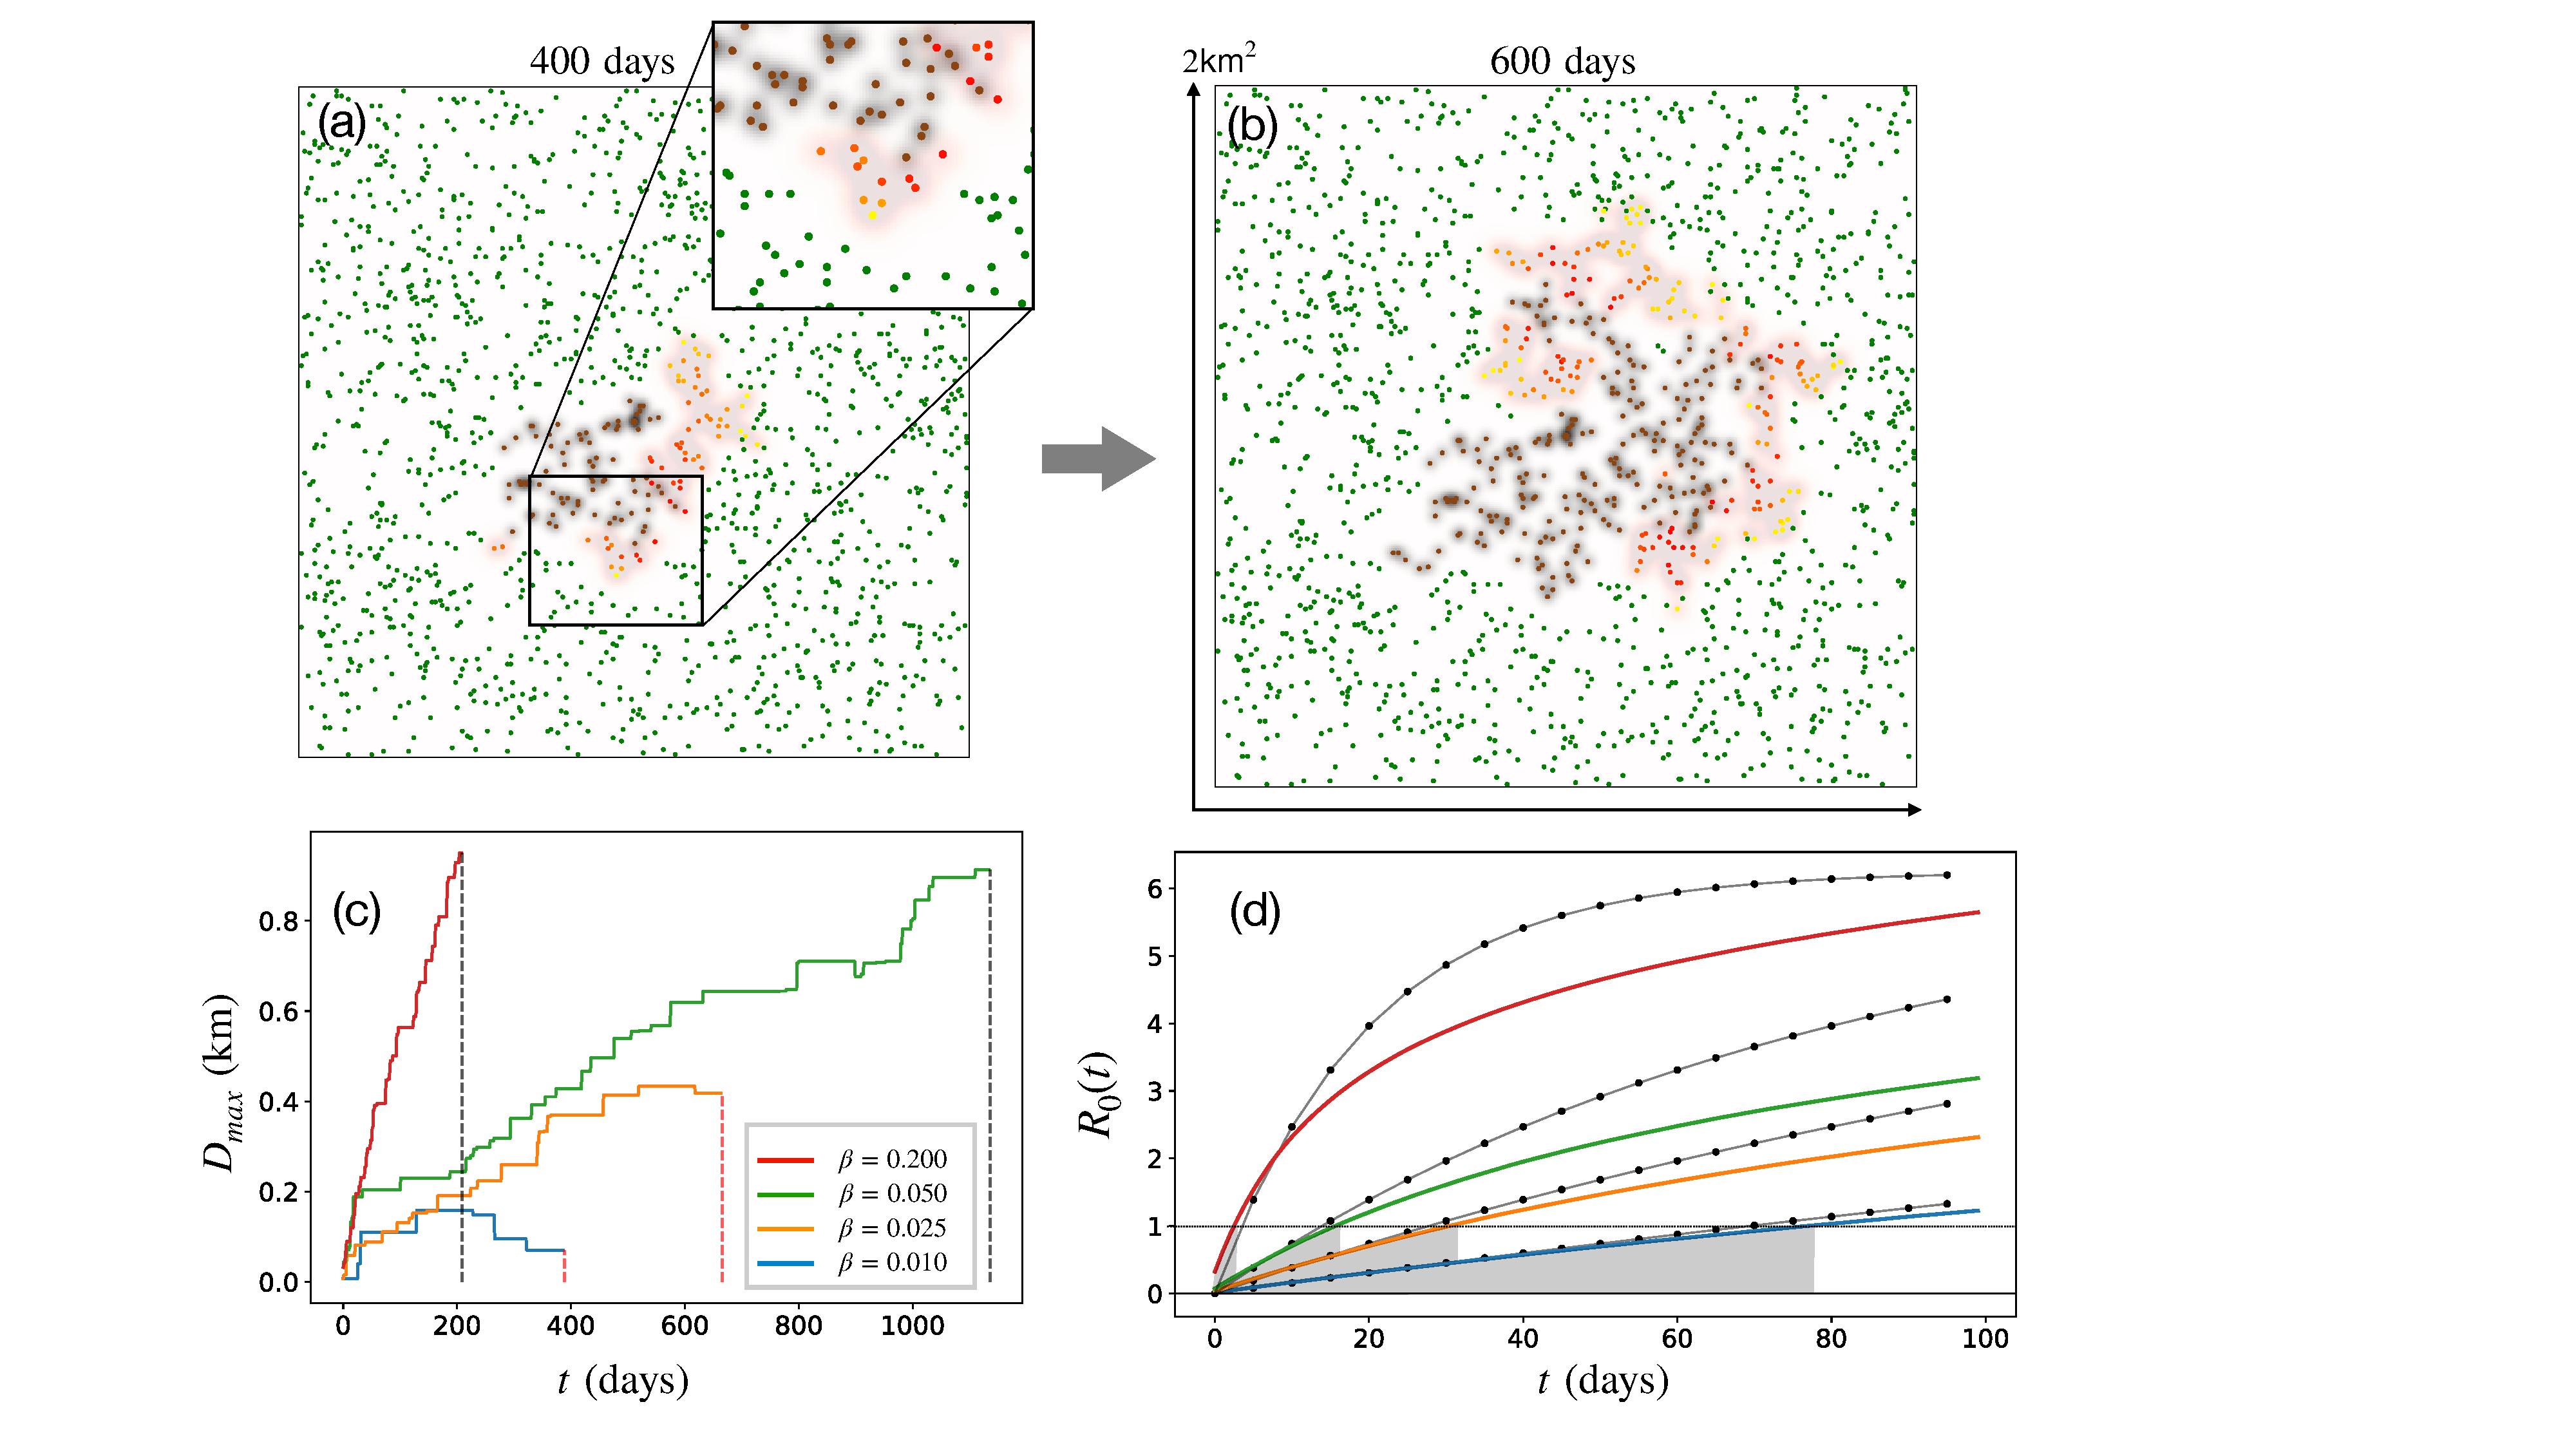
\includegraphics[scale=0.325]{chapter5/figures/figure1.pdf}
    \caption{Stochastic dispersal in the sub-grid model is shown through two time-steps of 400 (a) and 600 (b) days given parameters $\rho=0.01,\ \ell = 25\textrm{m}\ $ and $ \beta=0.05\ \mathrm{day^{-1}}$. Green pixels represent susceptible trees in $S$, while yellow and red pixels represent infected trees at different different steps in the $I$ category. Infected trees uniformly transition into the removed compartment shown in brown-black. (c) The time-series of maximum distance reached by an infected tree is shown for four typical simulations with parameters $\rho=0.01$, $\ell=25\textrm{m}$ and four variations infectivity. Vertical dashed red lines represent time-steps where the pathogen becomes extinct and dies while vertical black lines show when the pathogen survives to reach the domain boundary. (d) The mean number of secondary infections $R_0(t)$ is shown using the same model parameters as Fig \ref{fig:sgm-evol}(c). The black-dotted curves show the corresponding behaviour predicted from equation (\ref{eq:R0-final}).}
\label{fig:sgm-evol}
\end{figure}{}

After $t$ time-steps, the maximum distance reached by the pathogen is $D_{max}(t)$. This is found to be a useful metric that dynamically captures a pathogen progressing through the domain. Using the same domain conditions as shown in Fig \ref{fig:sgm-evol}(a-b), the time-series of $D_{max}(t)$ are shown in Fig \ref{fig:sgm-evol}(c) for a single simulation run and four variations of $\beta$. The time-series of $D_{max}(t)$ indicate if the pathogen becomes extinct or propagates to the lattice boundary and survives, shown by the vertical red and black dashed lines respectively. Gaussian dispersal does not permit the pathogen to jump large discontinuous distances, therefore, survival to the boundary defines a connected cluster of infectious-removed trees spanning the domain\footnote{This behaviour in Fig \ref{fig:sgm-evol}(a-b) could be considered an approximation to percolation, given the finite size of $\mathcal{L}$.} representing a small-scale epidemic spreading locally.\\

% Introduce uses and quantities taken from sub-grid --> R_0
An `effective' reproduction number can be defined through the following thought experiment: consider a single (primary) infected tree surrounded by a random homogeneous distribution of susceptible neighbours. Over the course of it's infectious life-time, the primary infection will lead to $R_0$ secondary infections. If secondary infections are not permitted to produce tertiary infections, the neighbourhood around the primary infection remains untouched by other diseased trees and the reproductive potential of the pathogen can be approximated by $R_0$. This can be directly simulated in a straightforward manner through ensemble-averages of the model.\\

A simplified approximation of the total number of secondary infections, after $T$ time-steps can be shown to be:
\begin{equation}
    R_0(T) = \rho_0 \mathcal{L}^2 \Big[ 1 - \exp(-\frac{2\pi\beta\ell^2}{\mathcal{L}^2}T) \Big]
\label{eq:R0-final}
\end{equation}{} 
% In a more realistic sense R_0 would include weather variability...
where $\rho_{0}$ is the tree density at time $t=0$. The formula does not take into account the spatial variation of transition probabilities (due to Gaussian dispersal) and approximates secondary infections to follow from dispersal of the form $g(r) = c$, where $c$ is a constant. A more accurate, albeit more complex, formula can be derived allowing for Gaussian spatial variations (see Appendix A). Realistic descriptions of the pathogens reproductive potential would take into account additional factors such as weather conditions, habitat suitability \cite{large-scale-model-SSTLM}, geometrical properties of the wave-front and long-range dispersal. However, in the current analysis we continue to use the simplified Gaussian approximation.\\

In Fig \ref{fig:sgm-evol}(d), the ensemble-averaged number of secondary infections is determined for each time-step $t\in [0, T]$ and plotted in a time-series $R_0(t)$. The time-series show four variations of $\beta$ alongside the dashed curves predicted by equation (\ref{eq:R0-final}). The final value of $R_0$ is observed when the infectious life-time is concluded. Lower $\beta$ values give a linear relationship which agree well with equation (\ref{eq:R0-final}). Here, linearity reflects a constant transition rate into the $I$ compartment as the neighbourhood fails to become saturated with infected trees. For progressively higher infectivities the number of secondary infections begin to plateau as less trees in the neighbourhood are available to infect.\\

From the effective reproduction number, a transmission threshold is defined by $R_0=1$, illustrated in Fig \ref{fig:sgm-evol}(d) by the grey horizontal line. When model parameters satisfy $R_0>1$, the pathogen may either propagate for a time before dying off (as demonstrated by the blue and orange time-series in Fig \ref{fig:sgm-evol}) or continue indefinitely\textemdash indicating an epidemic. For $R_0<1$, the pathogen has little chance of spreading to neighbouring trees and zero chance of culminating in an epidemic through the domain\protect\footnotemark \footnotetext{A stable epidemic regime through the domain $\mathcal{L}$ required parameters slightly above the transmission threshold. See \cite{R0-perc-ref} for a related discussion on the `final epidemic size' and reproductive ratios.}.\\

\subsection{Ash density distributions}
\label{section:data-rescale}

% Introduce the data set and re-scaling
The Ash abundance distribution reported by \cite{hill.data} had a resolution of $\mathrm{1km^2}$ and units of hectares of canopy cover per kilometer-squared of land. To ensure the abundance distribution was compatible with the sub-grid model we re-scaled the raw abundance values into a dimensionless tree density i.e. kilometer-squared of Ash cover per kilometer-squared of land. This was achieved by multiplying the data with an appropriate scale-factor, pixel values then become equivalent to the sub-grid density $\rho$. The re-scaled Ash distribution is shown in Fig \ref{fig:data-sources}(a) along with the density frequency distribution in Fig \ref{fig:data-sources}(b). Between the limits of $\rho \in [10^{-2}, 10^{-1}]$, the frequency distribution follows a power law of the form $\sim \rho ^{-k}$, as evident from the linearity on the logarithmic inset axes. The distribution had a fitted exponent of $k=1.90$, shown by the dashed black line. Intriguingly, this observation is suggestive of self-similarity in the data.

 \begin{figure}
    \centering 
    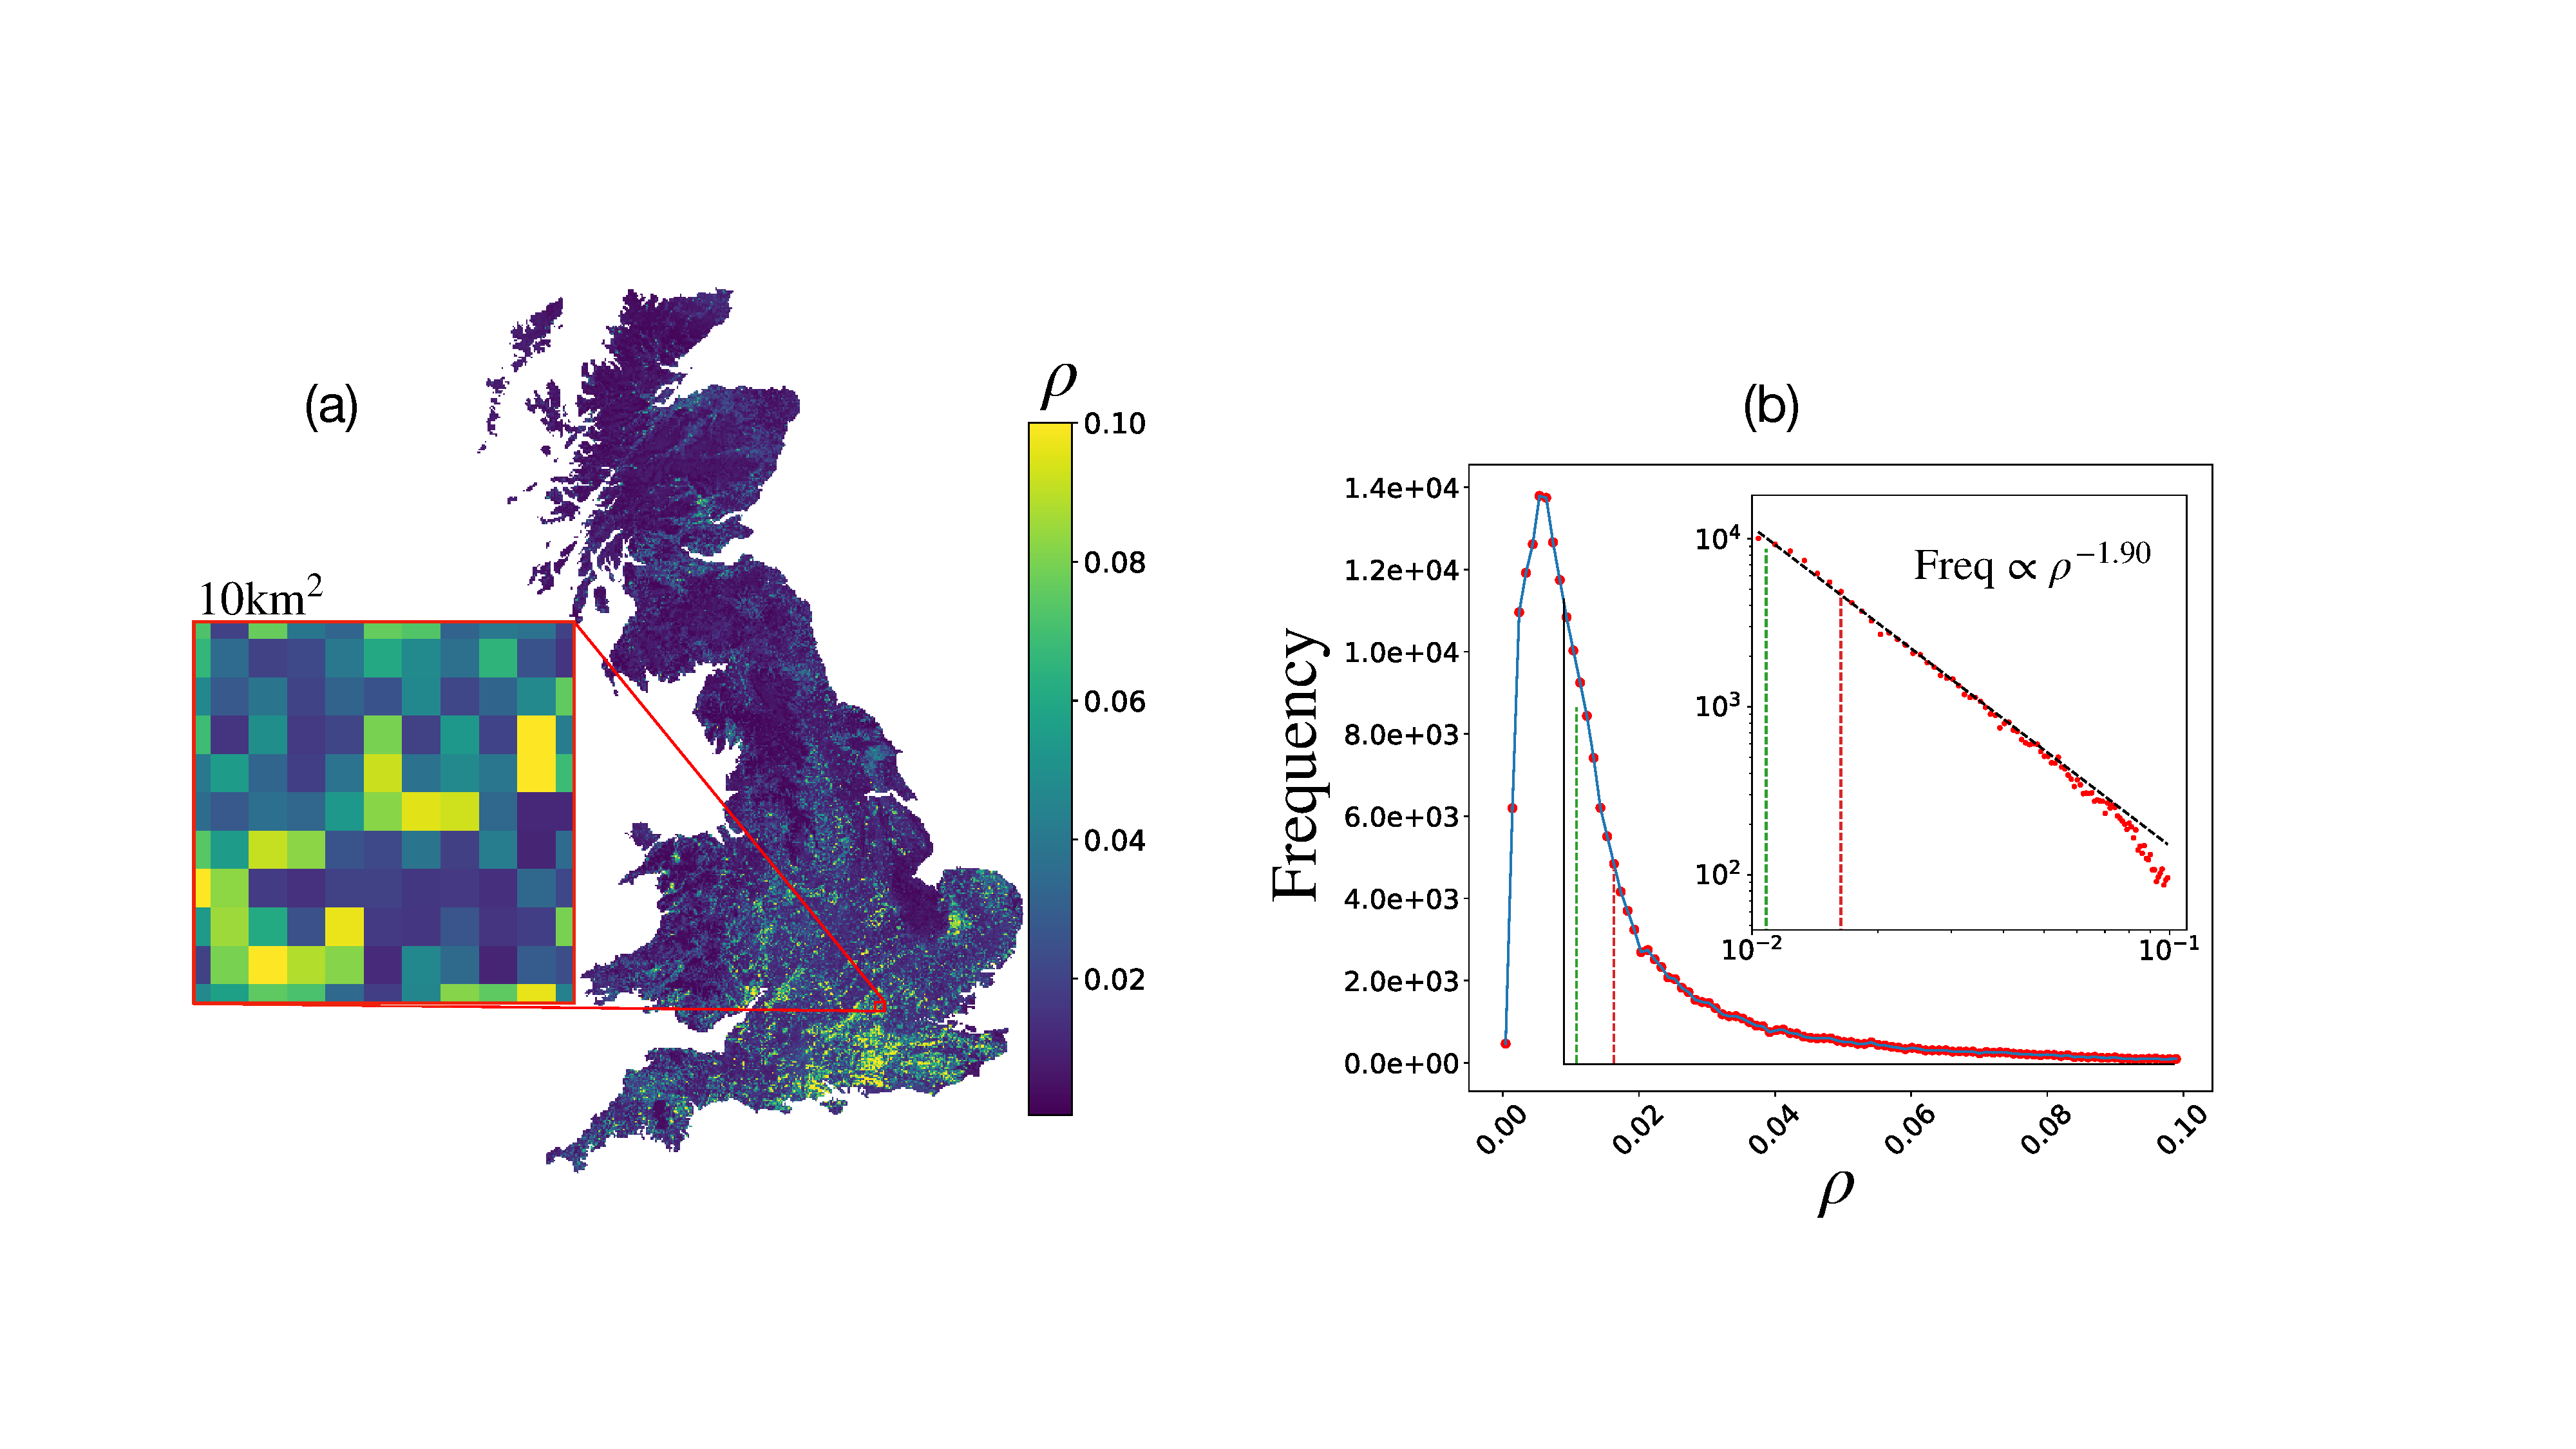
\includegraphics[scale=0.3]{chapter5/figures/figure2.pdf}
    \caption{(a) The abundance distribution of Ash as reported by \cite{hill.data} re-scaled into a tree density map. The zoomed inset shows $\mathrm{10 km^2}$ region. (b) The frequency distribution of tree density with inset showing the data on a log-log plot. Vertical green and red lines show median and mean tree densities respectively. The inset plot reveals that part of the frequency distribution follows a power law of the form $\sim \rho^{-k}$ with the fitted exponent taking the value $k=1.90$.}
    \label{fig:data-sources}
\end{figure}{}

\section{Results}

\label{section:results}
% Figure of ensemble results of sub-grid model
\subsection{Sub-grid ensemble behaviour}
\label{section:sgm-map-gen} 

% detail ensemble simulation results of the sub-grid
Understanding stochasticity within the sub-grid model necessitated an ensemble approach (of at minimum $10^3$ repeats) to categorize model behaviour. An ensemble of simulations produce a distribution of $R_0$ values. Four distributions are shown in Fig \ref{fig:sgm-ens}(a) for increasing tree densities. For each increase in $\rho$, the ensemble mean is calculated, denoted by $\langle \overline{R}_0 \rangle$, and shifts to higher values indicated by the vertical dashed lines. This permits the transmission threshold (mentioned in Section \ref{section:sgm-expo}) to be better described by $\langle \overline{R}_0 \rangle = 1$ and is used as a simplified criterion to distinguish between epidemic and extinction.\\

Figure \ref{fig:sgm-ens}(b) shows the ensemble mean $\langle \overline{R}_0 \rangle$ over a two dimensional parameter space of dispersal distance $\ell$ and infectivity $\beta$ with a fixed density $\rho=0.01$. Using equation (\ref{eq:R0-final}), the predicted transmission threshold is shown in orange. Numerical simulations generating values of $\langle \overline{R}_0 \rangle=1$ fell within $\pm 10\%$ of the orange line\textemdash due to stochasticity within the model. The threshold of transmission depends on the interplay of all the model parameters ($\rho, \ell, \beta$ and $T$). As the density increases trees become closer together, this lowers the values of infectivity and dispersal required before the pathogen can jump between trees.\\

\begin{figure}
\hfill
\centering
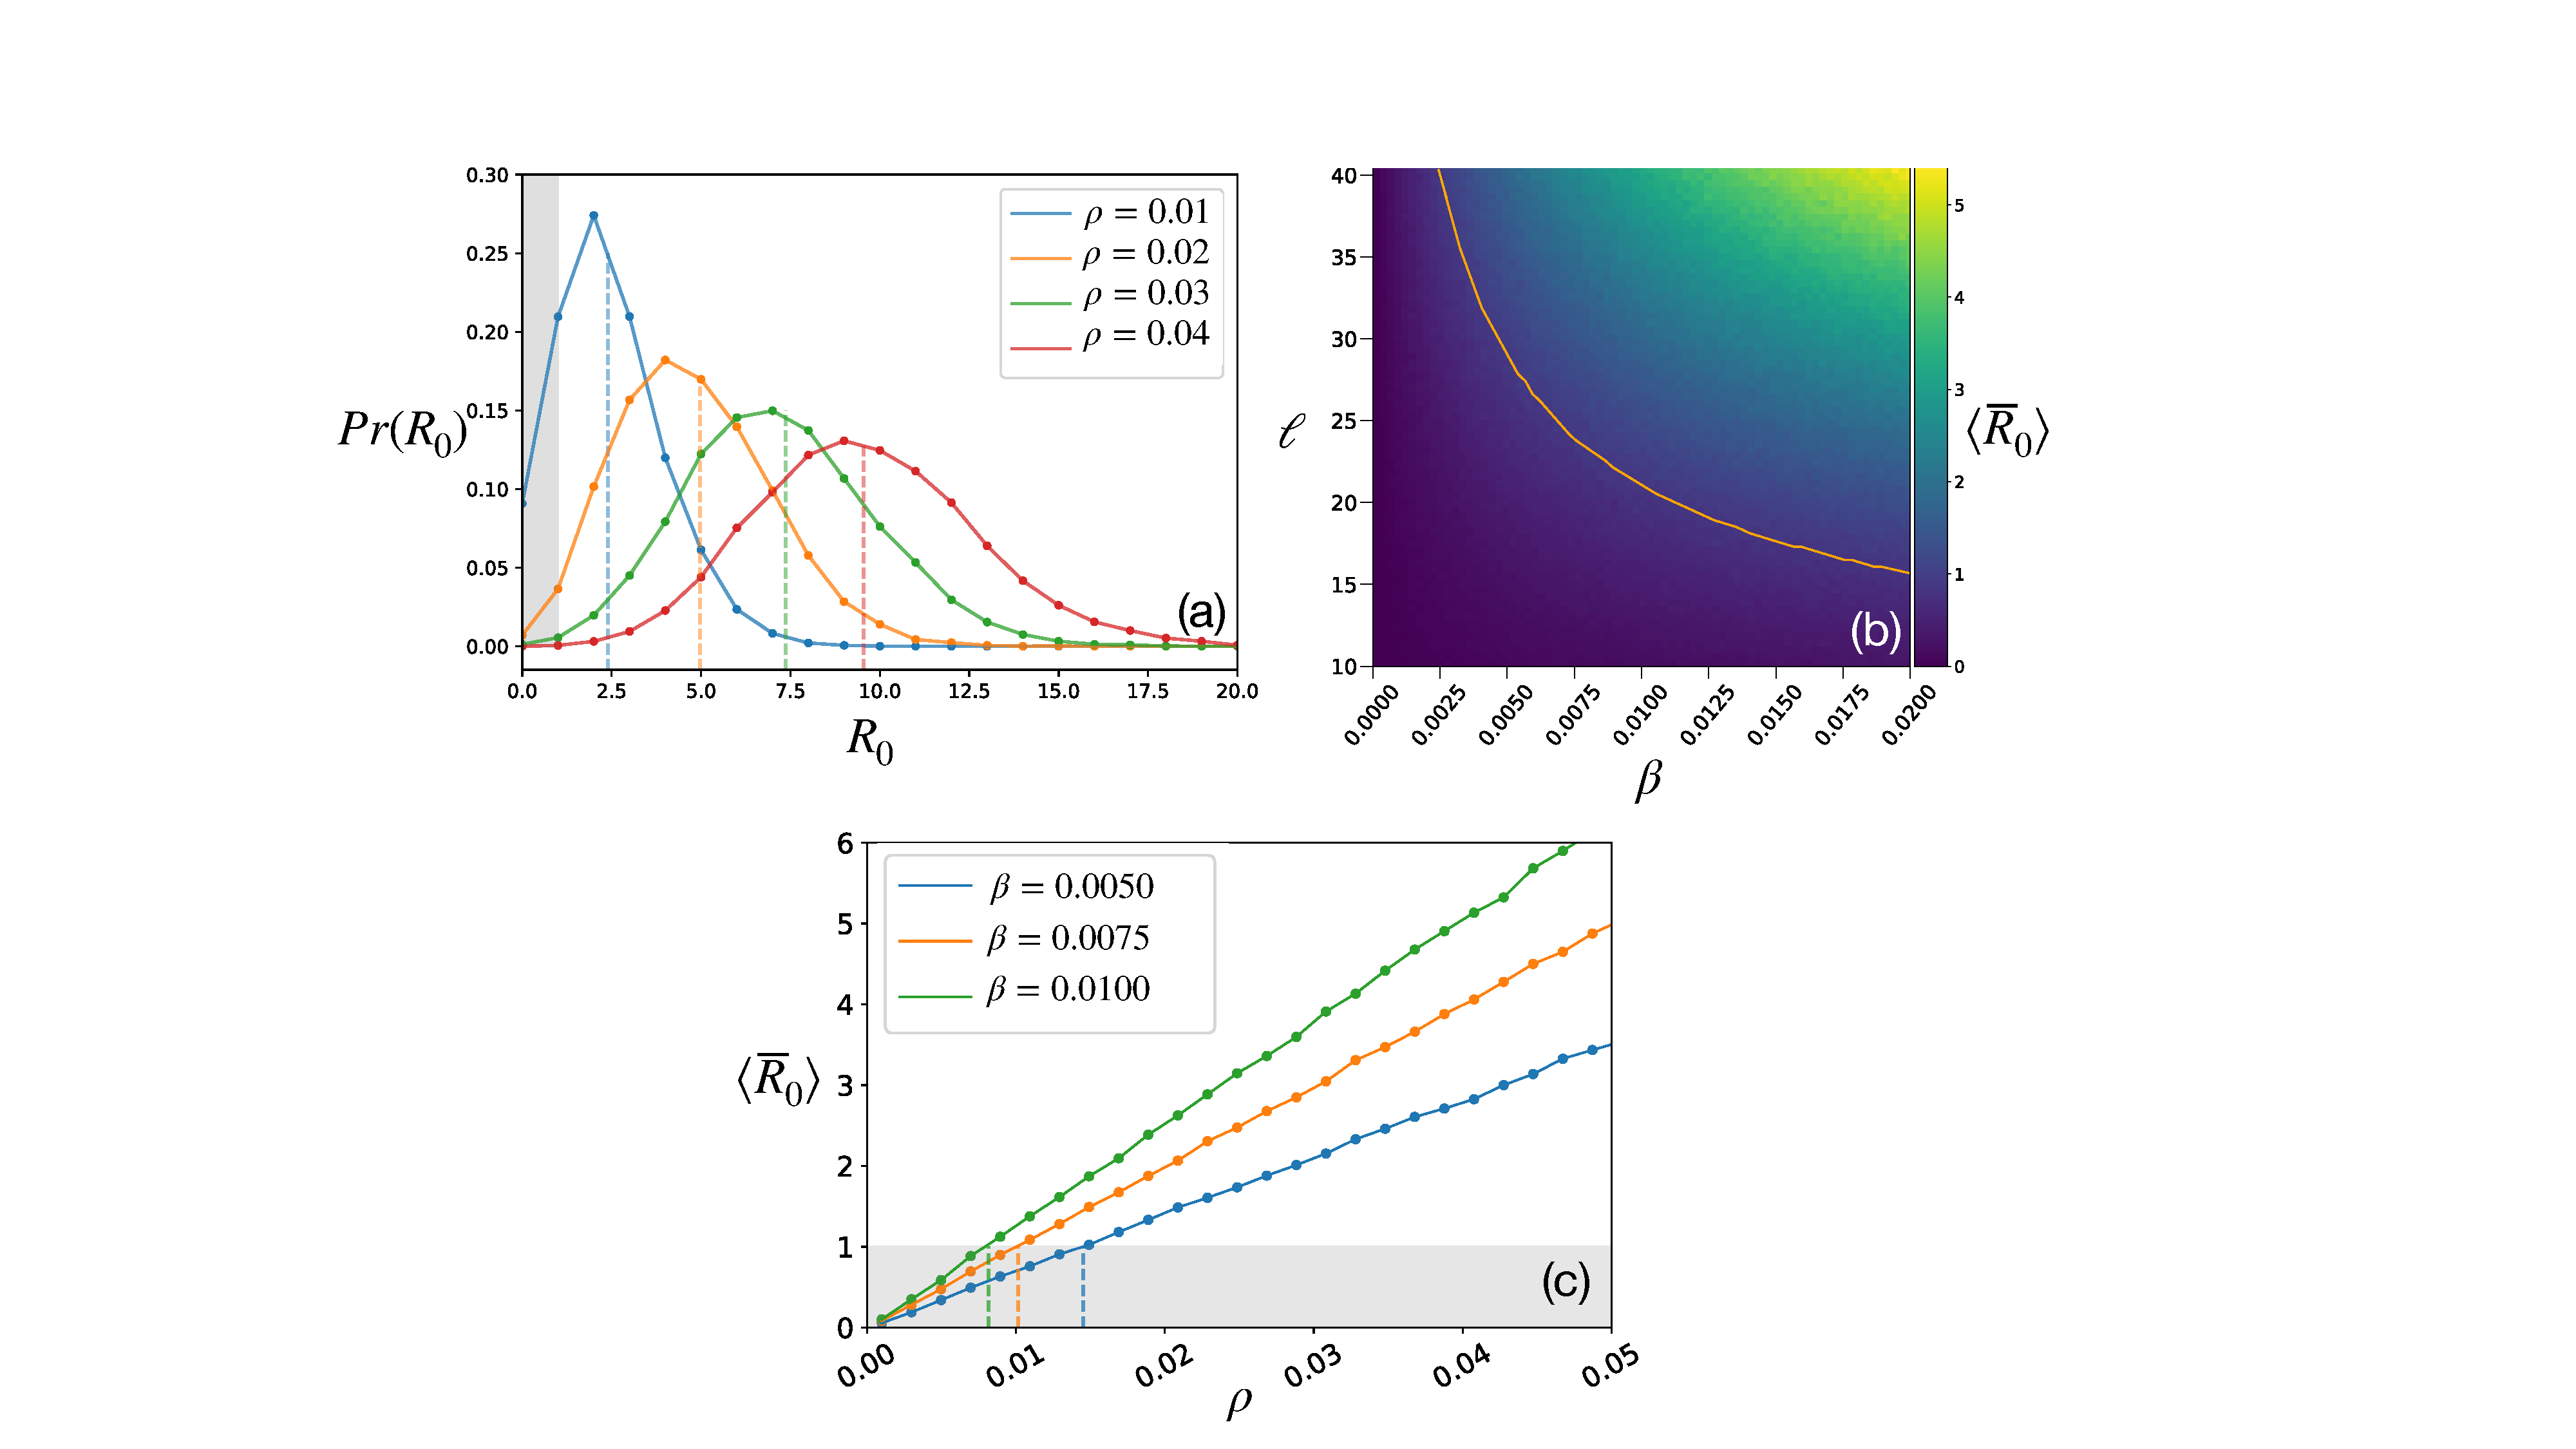
\includegraphics[scale=0.35]{chapter5/figures/figure3.pdf}
\caption{Ensemble behaviour of the sub-grid model. (a) An ensemble of simulations gives a distribution of $R_0$ values. The distributions for four $\rho$ values are shown with fixed dispersal and infectivity parameters $\ell=25\textrm{m}$ and $\beta=0.025\mathrm{day^{-1}}$. The ensemble mean $\langle\overline{R}_0 \rangle$ is shown by the vertical dashed line. (b) The ensemble mean is computed over the parameter space of dispersal $\ell$ and infectivity $\beta$ for fixed density $\rho=0.1$. The orange curve shows the transmission threshold $R_0 = 1$ predicted from equation (\ref{eq:R0-final})\textemdash numerical results fall within $\pm 10\%$ of the orange curve. (c) The mean effective reproduction number is shown as a function of $\rho$ for three variations of infectivity and fixed $\ell=25 \mathrm{m}$. Shaded regions show all values below the threshold $\langle\overline{R}_0 \rangle < 1$, the critical tree densities are shown by the vertical dashed lines.}
\label{fig:sgm-ens}
\end{figure}

A linear relationship between $\rho$ and $R_0$ is predicted by equation (\ref{eq:R0-final}), and this is confirmed by numerical simulations shown in Fig \ref{fig:sgm-ens}(c). For simplicity, the ensemble mean $\langle \overline{R}_0 \rangle$ will be referred to as $R_0$ from now on, unless otherwise stated. The regime of pathogen extinction is shown in shaded grey along with vertical dashed lines corresponding to the critical `density threshold' denoted by $\rho_c$  (equivalent to the threshold). When used in conjunction with the data-set from \cite{hill.data}, Fig \ref{fig:sgm-ens}(c) represents an appropriate projection of $R_0$ over the map of Great Britain.\\

\subsection{$R_0$-map generation and clustering}
\label{section:sgm-clustering}

% explain the linear-gradient method of R_0 generation
Figure \ref{fig:uk-mapping}(a) shows the  $R_0$-map generated with the sub-grid parameters $\beta=0.005\ \mathrm{day^{-1}}$ and $\ell=25 \mathrm{m}$. All proceeding results are based on these values. The choice of parameters, identical to those in the blue line of Fig \ref{fig:sgm-ens}(c), portray an arbitrary pathogen. All locations below the transmission threshold were presumed disease-free and given numerical values of zero (depicted by inland white-space). All values of $R_0$ over and above the threshold were taken as susceptible. Under the action of a more infectious pathogen, the $R_0$-map would be more dense as additional patches of land become susceptible.\\

In Fig \ref{fig:uk-mapping}(a), we can begin to identify heterogeneity and high-risk clusters of Ash. However, visualising which pixels connect to form large clusters is non-trivial. An image processing technique, `connected component analysis' (or CCA) \cite{CCA1, CCA2}, was used to identify and label susceptible clusters and simplify the $R_0$-map. This was performed using the function `label' from the Python-SciPy package `ndimage' \cite{scipy}. Doing so classified all susceptible (Moore) neighbours as connected members of the same cluster. Figure \ref{fig:uk-mapping}(b) shows the top 10 largest $R_0$-clusters found in the map of Fig \ref{fig:uk-mapping}(a).\\

% Interpretation of clusters
In this simplified interpretation, clusters represent a connected medium of Ash capable of supporting an epidemic, whereas regions below threshold act as barriers that inhibit the spread. Provided there is no long range dispersal (over $\mathrm{1km}$), a pathogen will not jump between clusters and will remain localised. Epidemic impact in this model will therefore correlate closely to cluster size as only large clusters have the potential of tending towards a nationwide spread of disease. Subsequent analysis will therefore concentrate on the largest susceptible clusters of Ash.\\

% Linking R0 clusters to percolation theory
The structure of connected $R_0$-clusters can be considered through the lens of a `\textit{percolation-like}' theory: if the $R_0$-map were homogeneous, a minimum number of susceptible (or `open' in percolation theory) positions defines a critical density. At the critical density, a `spanning' cluster is realised and percolates through the domain. In Fig \ref{fig:uk-mapping}(b), this picture is complicated by heterogeneity. Subsequently, we found connectedness inside a given cluster could depend on just a small number of `connecting points' which if removed, thinned below $\rho_c$, would lead to significant fragmentation and divide the cluster\footnote{An analogy to this idea can be found in the study of `conductive-insulator' percolation networks, with so called `\textit{hot-bonds}'. If broken, a \textit{single} hot bond can prevent the whole system from conducting \cite{RevModPhys.45.574, Herrmann_1984, hot-bond}. Although, in our analysis, a generalisation of this analogy is presented to include a set of \textit{multiple} hot-bonds.}.\\

\begin{figure}
\hfill
\centering
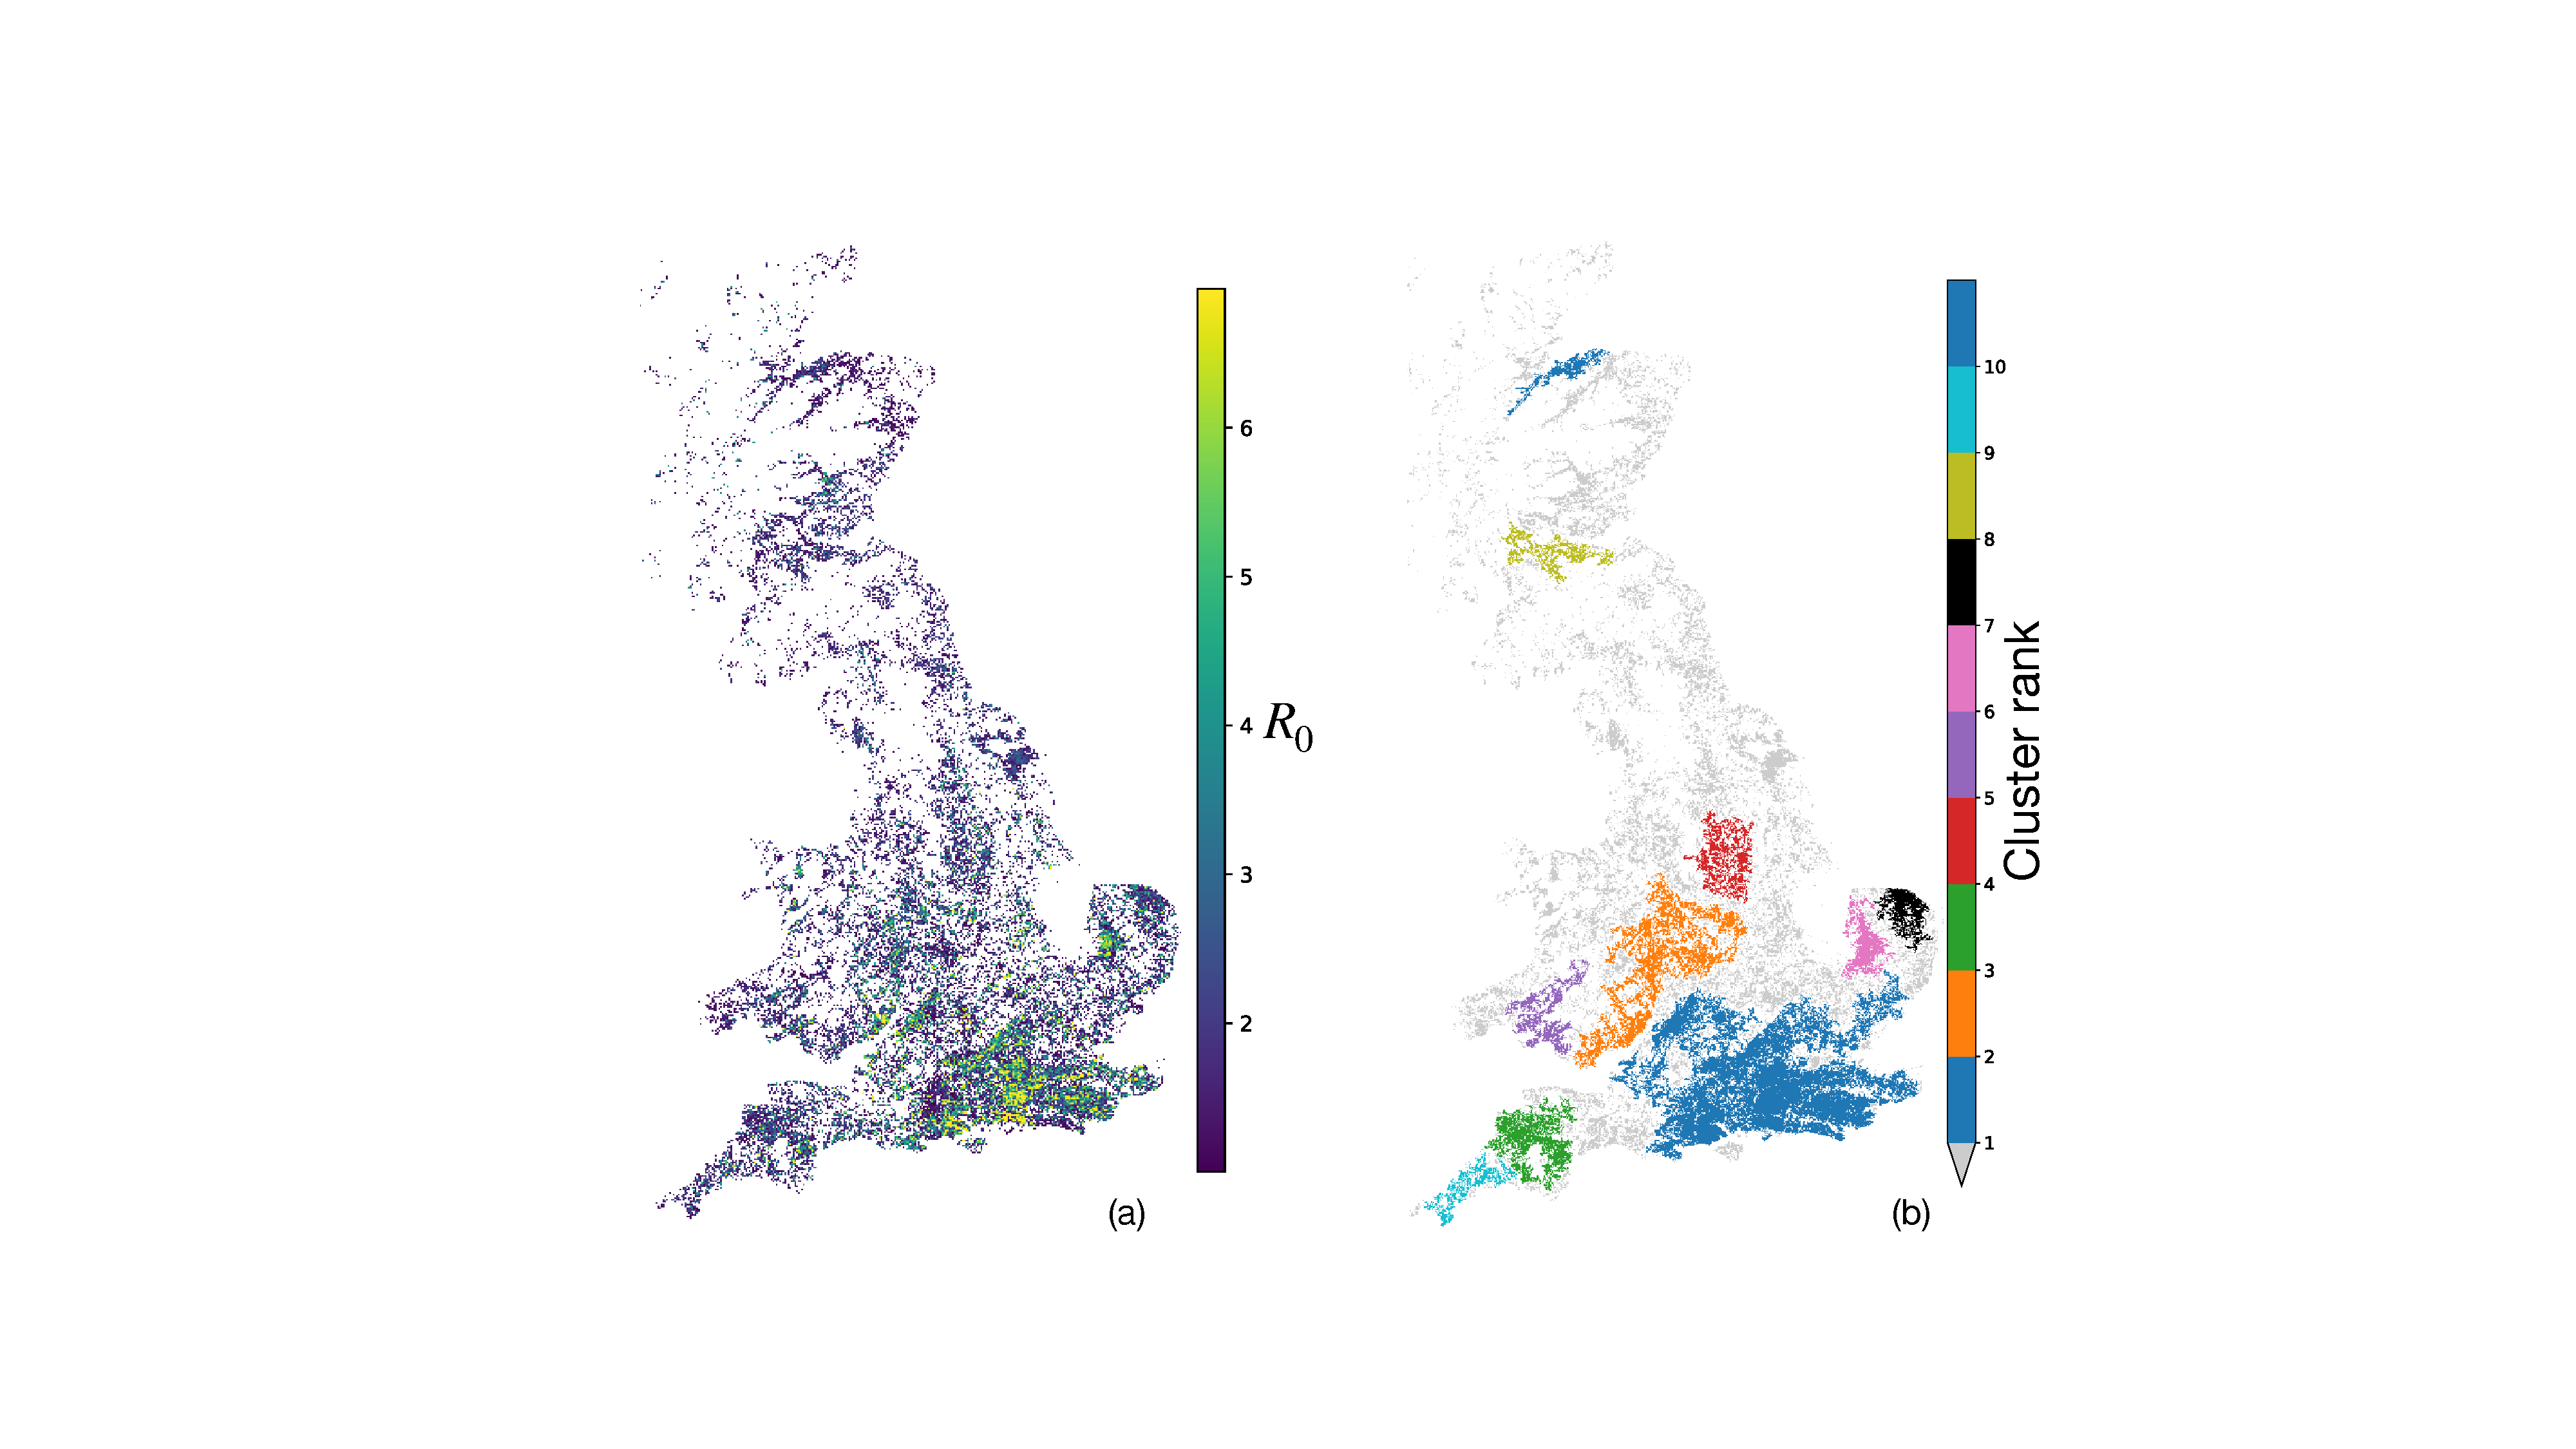
\includegraphics[scale=0.45]{chapter5/figures/figure4.pdf} 
\caption{(a) The mean $R_0$ values are mapped onto the Ash distribution for pathogen parameters $\beta = 0.005\ \mathrm{day^{-1}}$ and $\ell=25\textrm{m}$. All pixels represent $\mathrm{1km^2}$ patches of Ash with their predicted $R_0$ numbers\textemdash shown by color. Patches of Ash below the $R_0$ threshold are shown by inland white-space. (b) Using connected-component analysis, the top $10$ largest clusters of Ash are identified and ranked. Large connected regions identify high-risk areas of Ash in Great Britain.}
\label{fig:uk-mapping}
\end{figure}

Strictly speaking, the comparison with percolation theory breaks down on account of clustering in the $R_0$-map. That is, the susceptibility of a given pixel is likely dependent on its neighbours $R_0$-value. This contradicts classical percolation theory where lattice points are not correlated but exist independently of one another\textemdash much like the random-homogeneous distribution of trees presented in Section \ref{section:sgm-expo}. We precede by describing how these findings can be used to achieve efficient regional containment of an epidemic.\\

\subsection{Regional containment}
\label{section:optimal-culling}

Each cluster (denoted by $\mathbf{C}$) detected in the $R_0$-map represents a connected network of susceptible Ash where pathogen survival and spread is possible. The shape of each cluster is constrained by landscape topography and geography. If no control is attempted, all trees within a cluster are put at risk if one point in the cluster becomes infected. Given this, a control strategy is formulated by noting that removing specific positions of Ash (or breaking critical `links') via selective tree felling would efficiently break the cluster into two fragments. A technical explanation of the fragmentation algorithm is given in Appendix B.\\

Cluster fragments define two disconnected `sub-clusters' (named $\mathbf{C_1}$ and $\mathbf{C_2}$). This eliminates risk for trees inside one sub-cluster and accomplishes control by regionally containing an epidemic inside a `confining cluster'. Ash trees inside the confining cluster are assumed to be removed by the pathogen while Ash trees inside the remaining sub-cluster survive and remain susceptible. If the number of felled trees is low in comparison to the number saved, then efficient control is achieved.\\

The notion of fragmenting a cluster $\mathbf{C}$ into two sub-clusters $\mathbf{C_1}$ and $\mathbf{C_2}$ may be repeated $N$ times to produce a set of disconnected sub-clusters. After each fragmentation, sub-clusters were ranked according to the Ash population size they contained. This allowed the largest sub-cluster to be targeted in the next iteration. Figure \ref{fig:result-cluster-reductions}(a) shows the largest cluster identified in the $R_0$-map (named $\mathbf{C_T}$) iteratively fragmented $N=5$ times culminating in six disconnected sub-clusters, depicted as the colour-filled regions from orange-green. The zoomed inset of $\mathbf{C_T}$ highlights the critically-connecting links found during each fragmentation.\\

\begin{figure}
%\begin{raggedleft}    %% not needed
\hfill
\centering
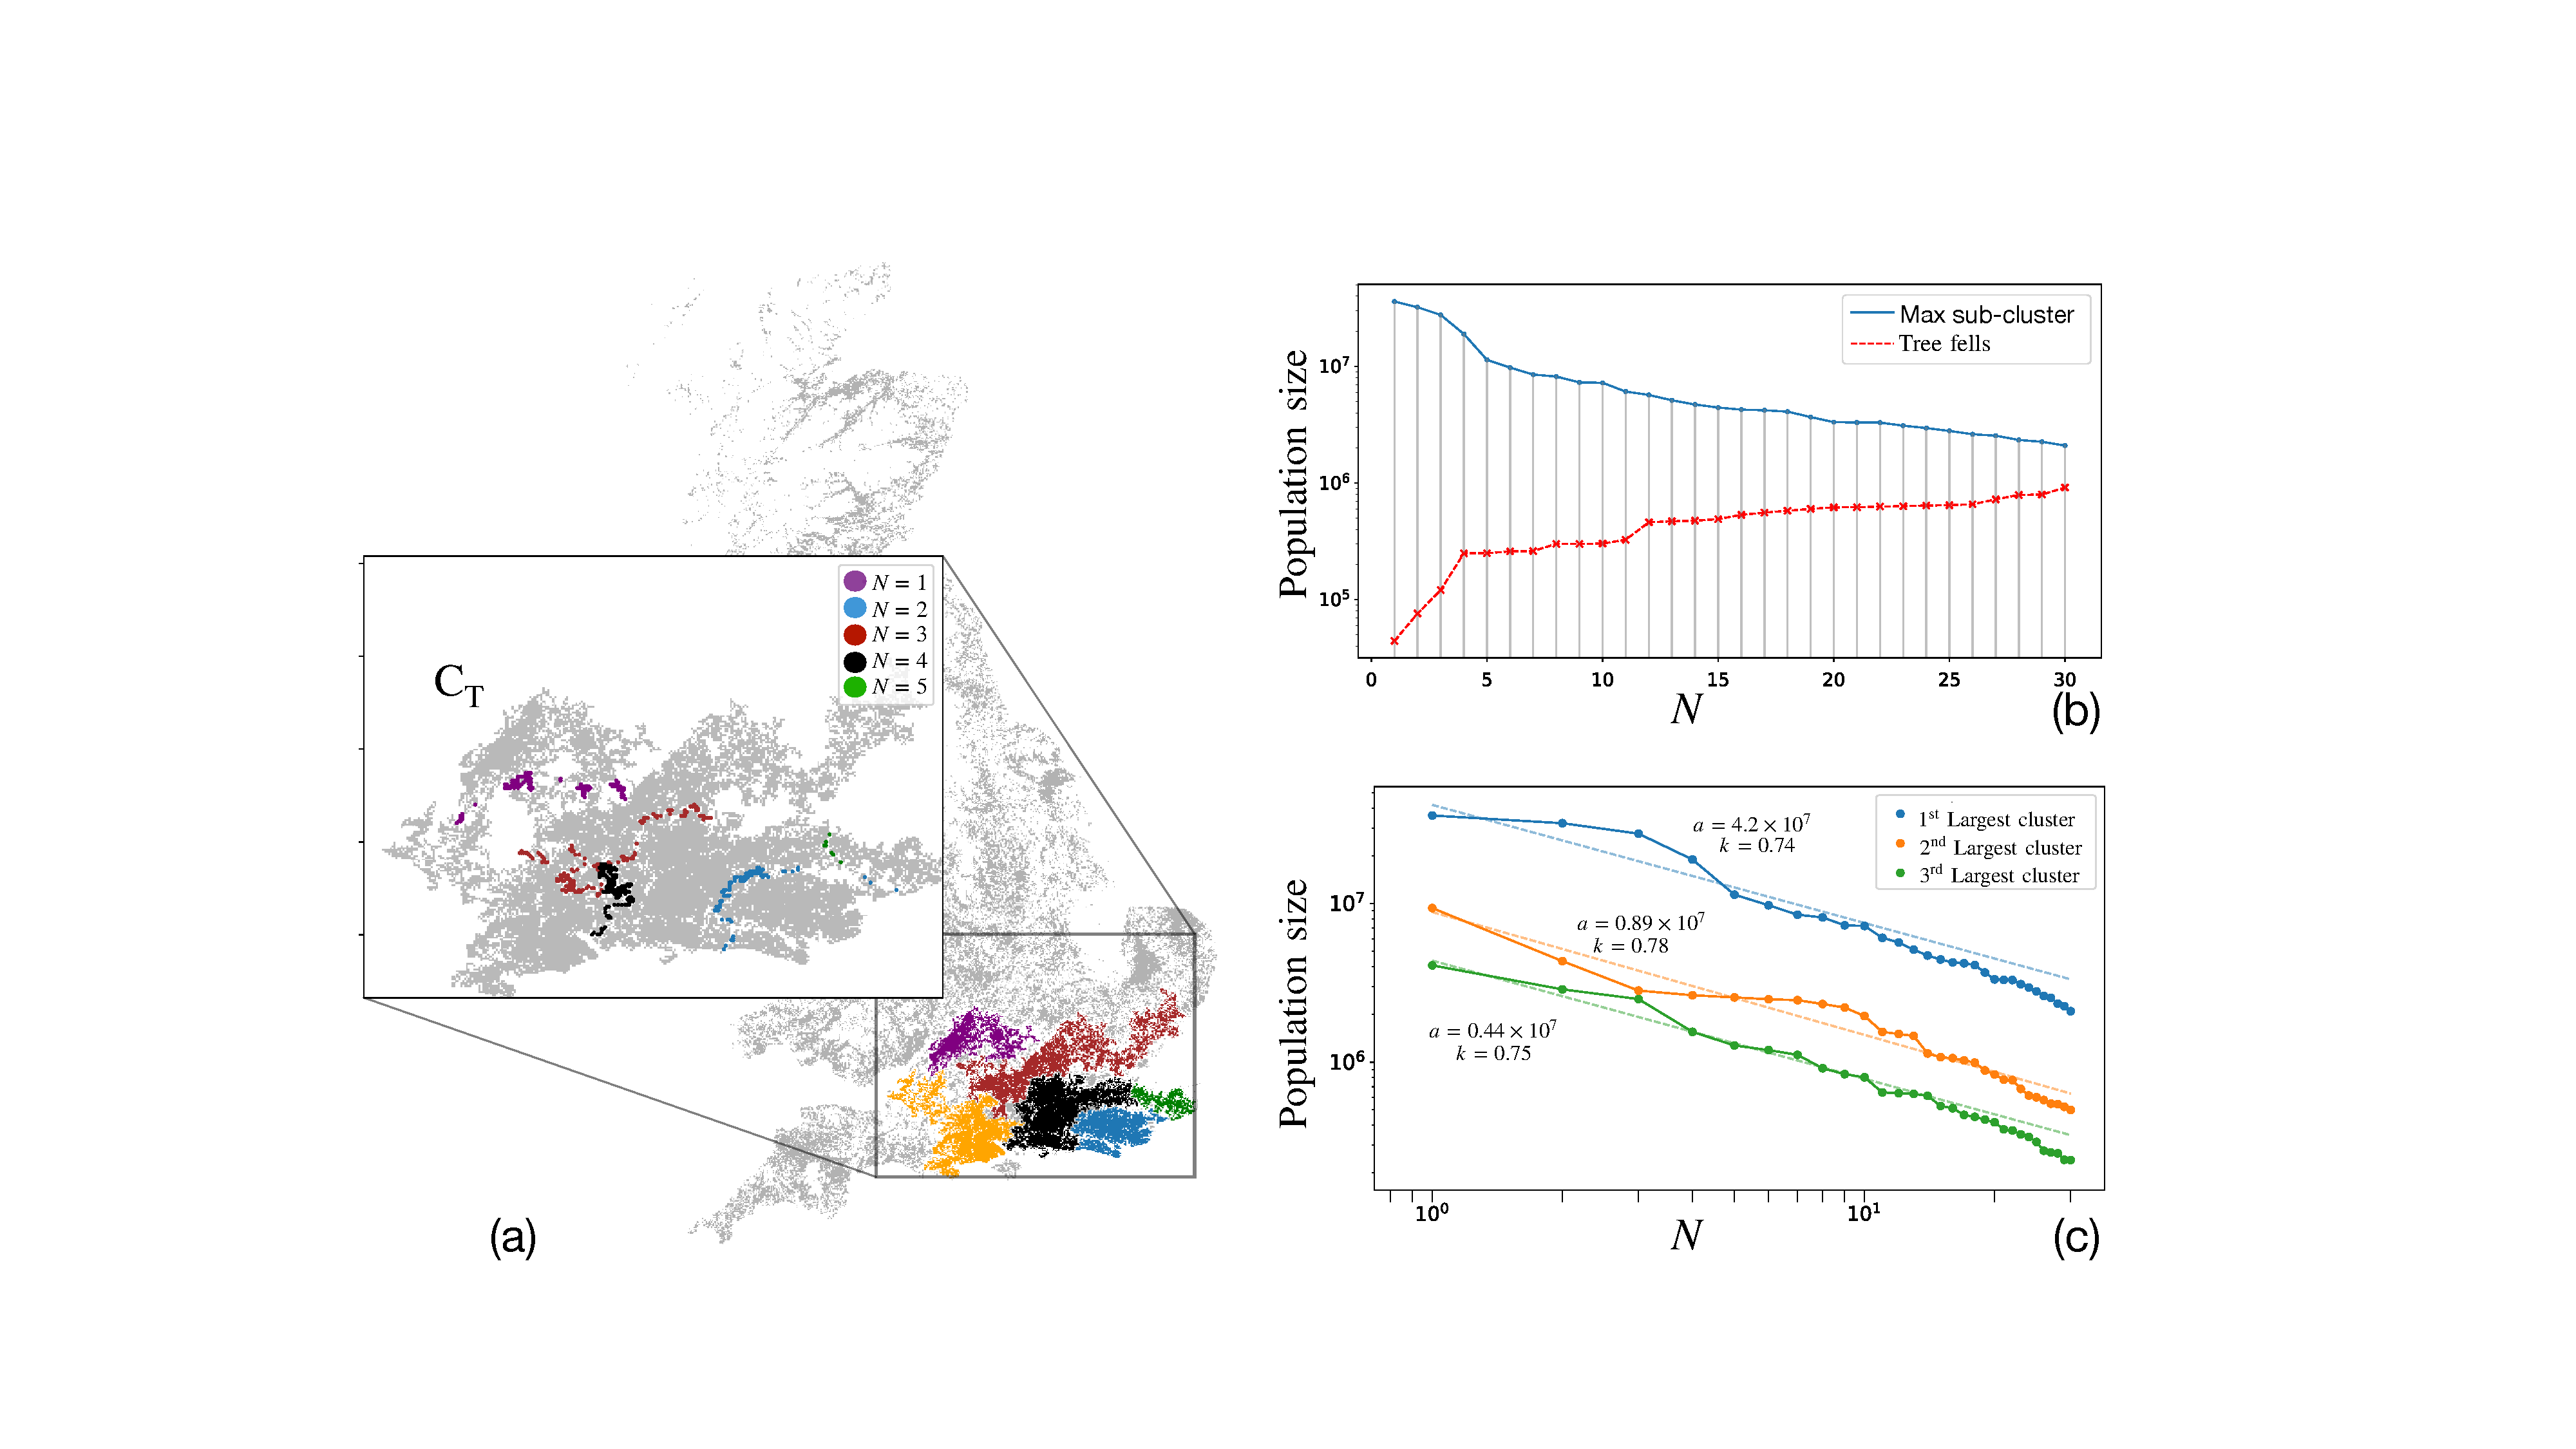
\includegraphics[scale=0.325]{chapter5/figures/figure5.pdf}
\caption{The fragmentation method is demonstrated on the highest risk clusters of Ash in the $R_0$-map. (a) The fragmentation method is iterated $N=5$ times on the largest ranked cluster in Fig \ref{fig:uk-mapping}(b) denoted as $\mathbf{C_T}$. The cluster is broken up into six disconnected sub-clusters shown by the colour-filled regions. The zoomed inset shows which critical links were identified in $\mathbf{C_T}$ for each cluster fragmentation. (b) Successively fragmenting the maximum sub-cluster inside $\mathbf{C_T}$ yields smaller sub-clusters, shown by the monotonically decreasing blue curve. The dashed red line shows the sum-total number of felled trees required for fragmentation. (c) Results of fragmentation are generalised to include the $\mathrm{2^{nd}}$ and $\mathrm{3^{rd}}$ largest ranked $R_0$ clusters in Fig \ref{fig:uk-mapping}(b). Results show cluster-size reductions on a logarithmic axes where fragmentation can be seen to follow a power-law of the form $f(x) = ax^{-k}$. Fitted parameters of $a,k$ are shown and plotted as dashed lines.}
\label{fig:result-cluster-reductions}
\end{figure}

We assume the average Ash tree in the population covers an area of $\mathrm{25m^2}$ (giving a maximum of $400$ trees per hectare of canopy cover \cite{ash-tree2, ash-tree1}). Combining this assumption with the data permits us to estimate the number density of Ash trees per point and subsequently the population size of Ash contained inside each sub-cluster. Additionally, an estimate towards the number of felled trees can be formed, thus giving insight into the scale of resource expenditure. This is achieved by first finding the difference between $\rho_c$ and the density values of critical links (i.e. the level of required density reductions), then multiplying this by the number density.\\

Figure \ref{fig:result-cluster-reductions}(b) shows the maximum sub-cluster population size in blue alongside the estimated number of trees needed to be felled in red. The largest sub-cluster continually decreased over $N=30$ iterations of fragmentation. Size reductions occurred more rapidly at first, starting from $\mathrm{3.5\times 10^7}$ trees and decreasing to $\mathrm{1.1\times 10^7}$ trees within $5$ iterations. By $N=30$, the rate of sub-cluster size reductions leveled off suggesting fragmentation in the field may tend towards diminishing returns on control efficiency. That is, larger values of $N$ produce smaller changes in the number of saved trees in proportion to the expenditure of resources needed to fell trees. This is demonstrated when the red and blue lines begin to approach each other, attaining comparable values.\\ 

In Fig \ref{fig:result-cluster-reductions}(c), sub-cluster size reductions in $\mathbf{C_T}$ are shown alongside the $2^{nd}$ and $3^{rd}$ largest $R_0$-clusters on a log-log plot\textemdash from solid blue through to green. The straight lines indicate a power-law. The sub-cluster size reductions were fitted to a power-law of the form $f(x) = ax^{-k}$, shown by the corresponding dashed lines. Fitted parameter values of $a$ and $k$ represent the initial cluster population size and rate of decrease respectively. Importantly, all sub-cluster size reductions demonstrate an exponent of $k\sim 3/4$. In addition to the Ash species shown here, Conifer (\textit{Pseudotsuga menziesii}) and Beech (\textit{Fagus sylvatica}) were given by \cite{hill.data} and were used comparatively to test fragmentation. For each species considered, all iteratively fragmented clusters had similar exponent values, $k\sim 3/4$.\\

\begin{figure}
    \centering
    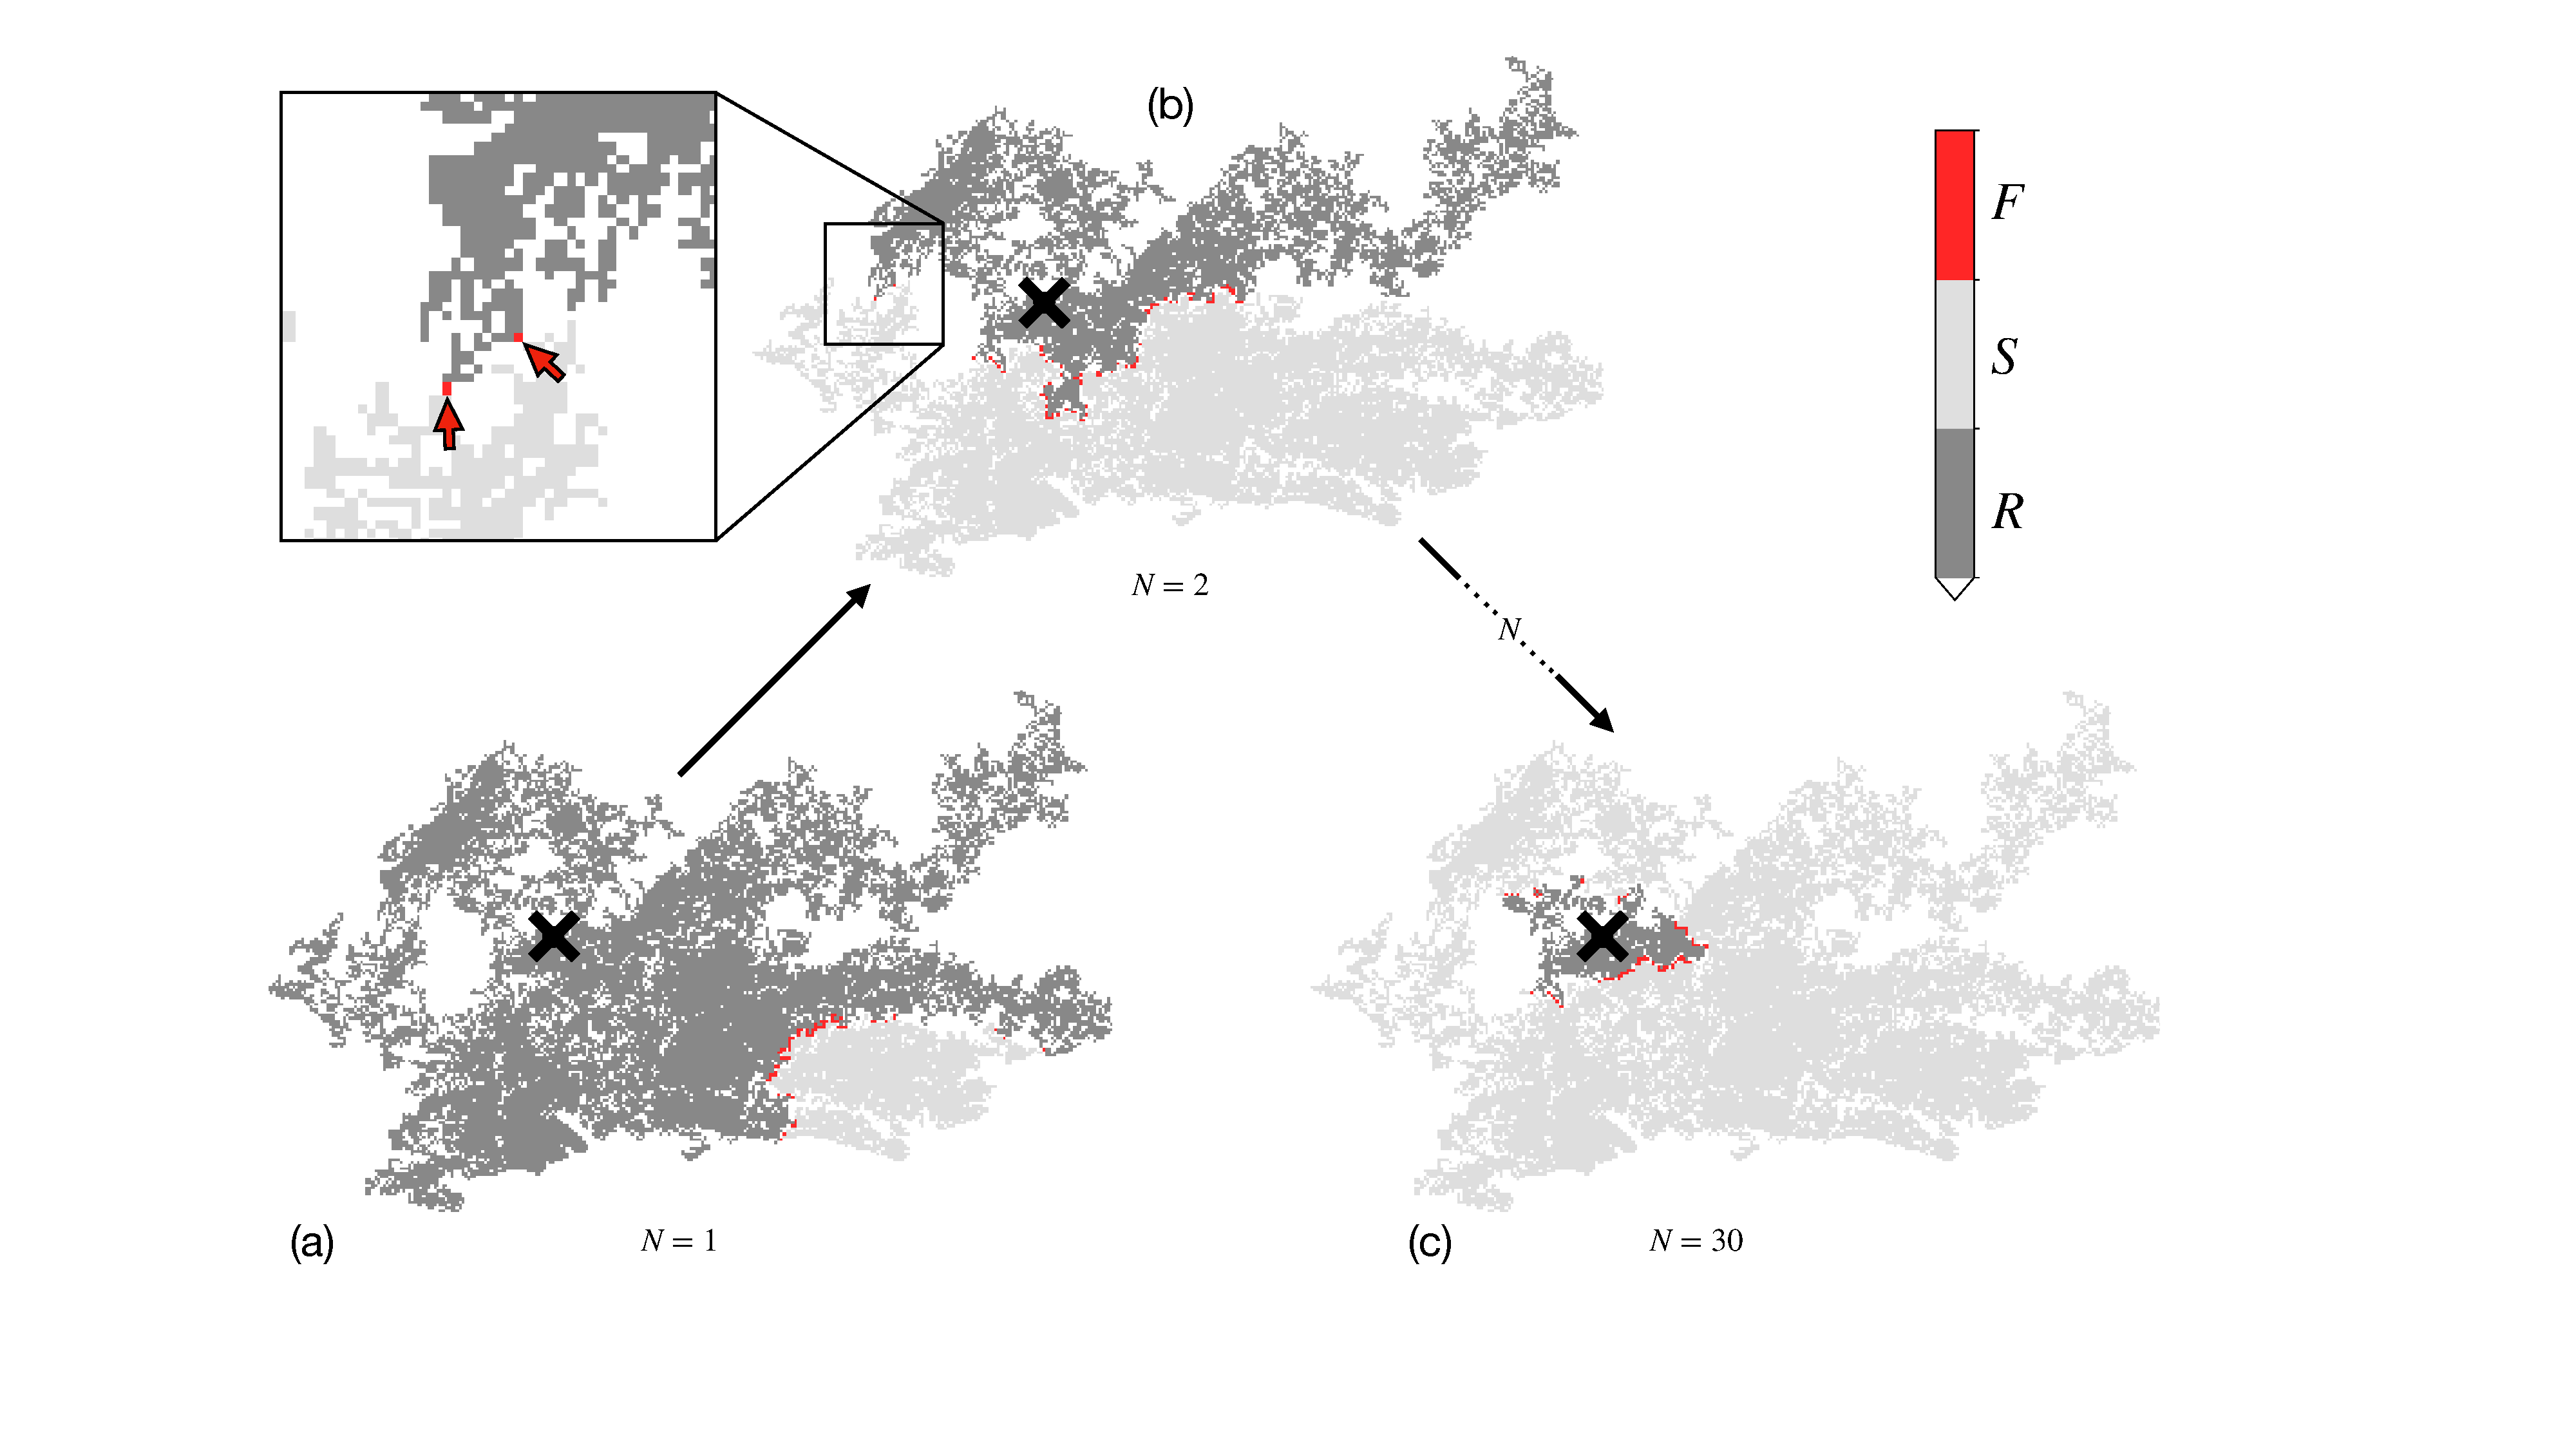
\includegraphics[scale=0.35]{chapter5/figures/figure6_.pdf}
    \caption{For each epicenter a variety of different felling choices can contain the epidemic. Here, an example is shown for an arbitrary epicenter depicted by the black cross as the number of cluster fragmentation iterations $N$ is varied. As $N$ is increased from $\mathrm{1}$ to a maximum of $\mathrm{30}$, new cluster fragmentations are produced and additional ways of confining the epicenter can be simulated. Regions that undergo felling ($F$) are shown in red. The sub-cluster containing the epicenter is considered removed ($R$), shown in dark grey. All other trees, shown in light grey, remain susceptible ($S$) and are saved from the epidemic. The zoomed inset depicts two points of contact in $F$ that separate parts of $S$ and $R$.}
    \label{fig:scenario-expo}
\end{figure}{}

\begin{figure}
    \centering
    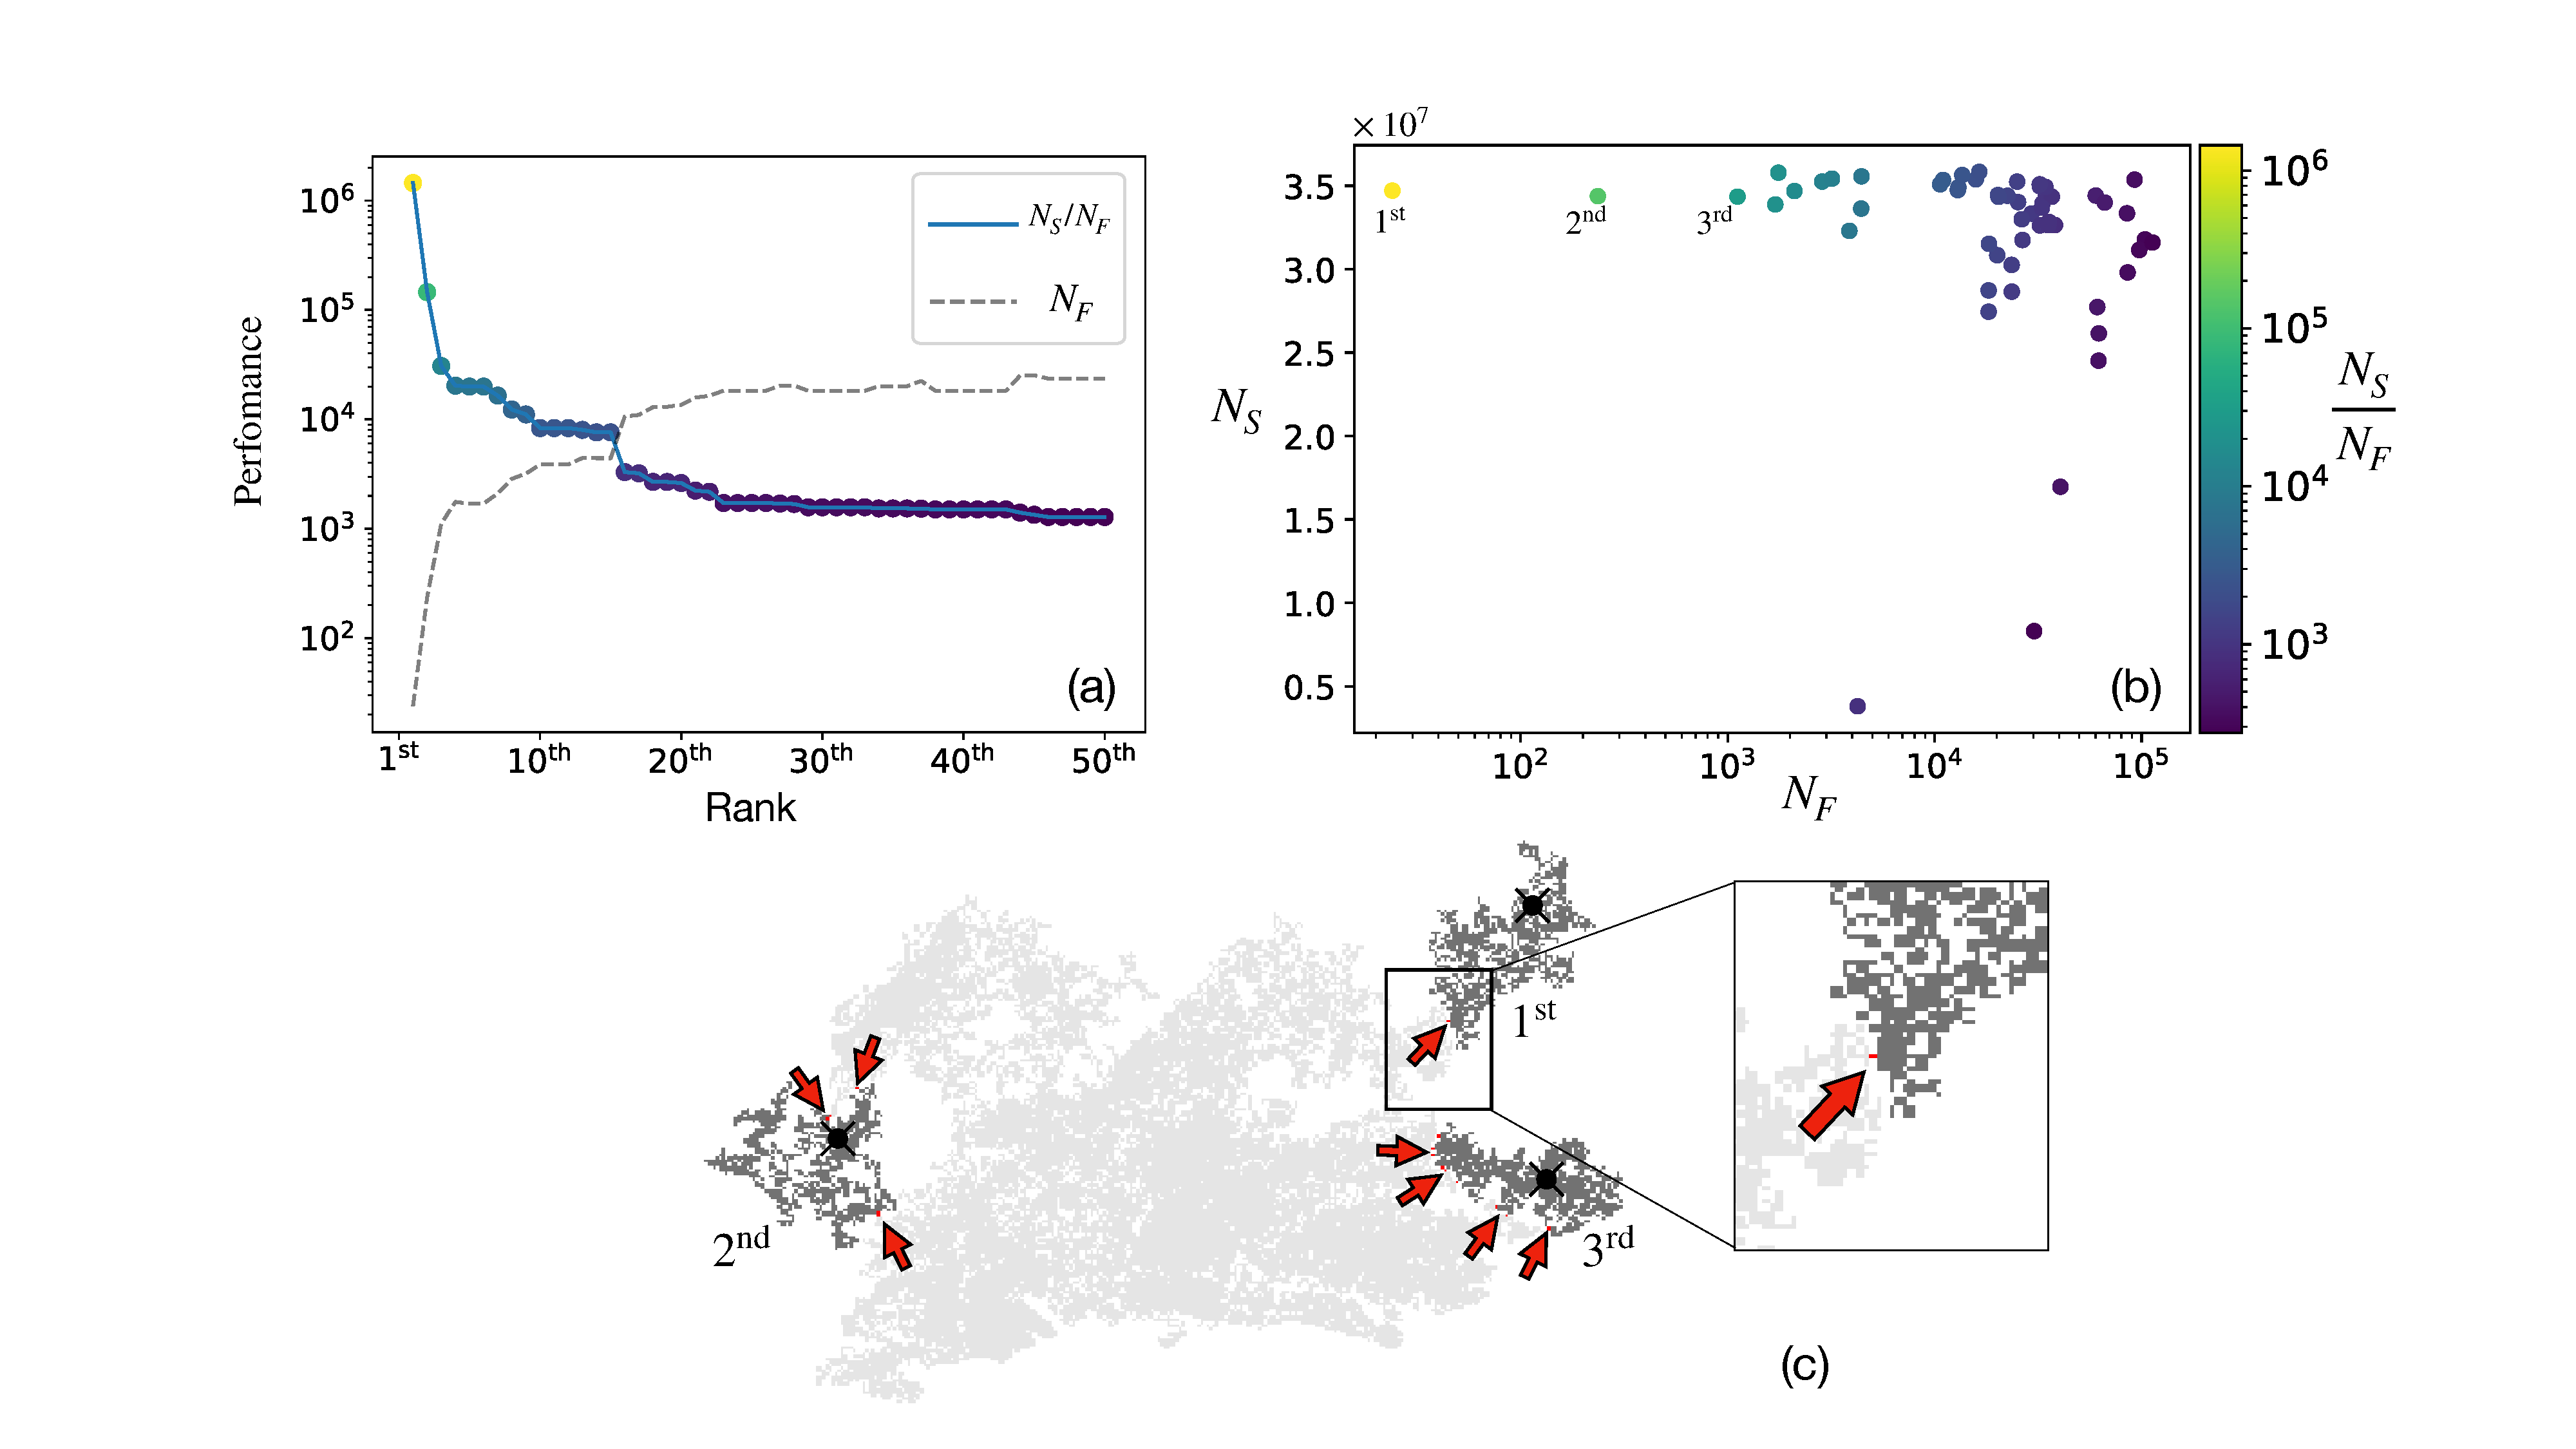
\includegraphics[scale=0.325]{chapter5/figures/figure7.pdf}
    \caption{(a) The top $50$ performing epidemic containment scenarios are ranked and plotted. The solid blue line (overlaid with colored scatter-plot) shows the payoff and reveals a small number of exceedingly high efficiencies. The dashed grey line contrasts the estimated number of trees felled. (b) The number of trees saved $N_S$ against the number felled $N_F$ is shown on a scatter plot and presented with a color map indicating the payoff ratio. (c) Out of all simulated epicenters, the $\mathrm{1^{st}, 2^{nd},\ and\ 3^{rd}}$ highest efficiency scenarios are spatially illustrated on the same map. Black circles represent epicenters and red arrows emphasise selected felling points for each cluster-fragment. The inset plot highlights the most efficient scenario, with just one point of contact involving just $2\times 1 \mathrm{km^2}$ patches of felled Ash felled.}
    \label{fig:result-culling-efficiency}
\end{figure}{}


\subsection{Epidemic control}
% Main results figure 7
Regional containment as a strategy of epidemic control was tested by considering outbreaks from different epicenters inside the target cluster $\mathbf{C_T}$. Starting from an epicenter, epidemic containment can be achieved in a variety of ways. Figure \ref{fig:scenario-expo} demonstrates this for a single epicenter marked by the black cross. The number of fragmentation iterations is varied from $N=1$ to $N=30$. For each step $N$, we identify which critical links, shown in red and denoted as $F$, should be felled below $\rho_c$ in order to define a confining sub-cluster around the epicenter. The population of saved Ash, illustrated in light grey, remains in state $S$ while all trees inside the confining sub-cluster, shown in dark grey, are assumed to transition into state $R$. By assessing the number of trees saved against the number of trees felled we can define a `payoff' ratio as $N_S/N_F$.\\

A set of epicenters were defined in $\mathbf{C_T}$ (by identifying the center of mass for each sub-cluster when $\mathbf{C_T}$ was iteratively fragmented $N=30$ times). From $31$ different epicenters and $30$ iterations, $930$ containment scenarios were simulated. For some epicenters, typically in close proximity, containment looked identical up to $N$ iterations before a different payoff ratio was registered. Subsequently, less than $930$ unique data-points between $N_S$ and $N_F$ were found\textemdash shown in Fig \ref{fig:result-culling-efficiency}.\\

The payoff ratios determined from the top $50$ performing containment scenarios were then ranked and plotted, shown in Fig \ref{fig:result-culling-efficiency}(a) by the blue line overlaid with a coloured scatter plot. For the purposes of our model, the payoff efficiency is shown alongside the corresponding number of felled trees in dashed grey. Payoff efficiencies begin to level off around $\mathrm{10^3}$ involving around $\mathrm{10^4}$ felled trees. In reality, this would be a challenge to accomplish in a reasonable time-frame. Fig \ref{fig:result-culling-efficiency}(b) shows a scatter plot of all the data, $N_S$ and $N_F$ are plotted with color corresponding to the payoff. The efficiency ranged over multiple orders of magnitude up to a maximum efficiency of $\mathrm{10^6}$. The top left quadrant of Fig \ref{fig:result-culling-efficiency}(b) represents viable scenarios where containment felling could be pragmatically implemented by policy makers with the greatest efficiency.\\

A small number of exceedingly high payoff results were found. In Fig \ref{fig:result-culling-efficiency}(c), the top three ranking payoff scenarios are illustrated on the same map and reinforces the intuitive notion that epicenters around edge positions can be most efficiently contained. The zoomed inset highlights just $\mathrm{2\times 1km^2}$ Ash patches located at a single point of contact for the top ranked sub-cluster. Critical links for the best performing scenarios were all found in lower-density regions within the $R_0$-cluster and were easily fragmented with a low number of felled trees. This highlights the possibility that fragmentation is most easily achieved with tree felling through critically linking regions and demonstrates how regional variation in host density can be exploited for efficient control.  

\section{Discussion}
\label{section:disscussion}
% summary of work 
We began our study by presenting a simple, small-scale, stochastic $SIR$ model of pathogen dispersal. Following this, an effective reproduction number $R_0$ was defined and used to quantify model behaviour. Pathogen dispersal relied on a generic Gaussian probability distribution. This could be adapted to specific pathogens with parameter and kernel fitting. Long-tailed (or hybrid multi-scale) distributions have been shown to be more realistic for both spores and insects \cite{long-range-dispersal}. Additionally, the $SIR$ compartments could be a generalised, the inclusion of an exposed category is one such example. Neglecting long-distance dispersal allowed us to approximate dispersal behaviour with a Gaussian kernel. Simplifying dispersal (along with having just three tree categories) helped to avoid over complicating the sub-grid model.\\ 

% Data choices and problems
Broadly speaking, host species data-sets are comprised of either binary-valued presence and absence or continuous-valued abundance distribution maps. Abundance data-sets measure the host canopy cover over each pixel. Owing to the large amounts of information captured inside each pixel they are useful for epidemiological models. Abundance data-sets are expensive to collect by conventional means, consequently they are in short supply over large regions. This is problematic for plant modellers and typical of insufficient and incomplete species distributions \cite{13-challenges}. We found the availability of suitable singe-species abundance data sources that cover large-scales to be sparse. To overcome this obstacle, a modelled abundance distribution of Ash in Great Britain \cite{hill.data} was chosen and provided a freely available realistic data source from which to develop the large-scale model of tree disease epidemics.\\

%R0 map and results
For an arbitrary pathogen, we explained how to generate epidemically relevant $R_0$-maps for Ash trees in Great Britain using the modelled abundance data. Simulating $R_0$ values directly from spatially explicit simulations proved computationally efficient owing to the linear relationship between $R_0$ and $\rho$. From the $R_0$-map, we explored a novel strategy of regional containment to accomplish epidemic control. The sub-grid approach captured small-scale stochastic interactions, between trees, that were used to produce the large-scale $R_0$-map; this is an attractive feature because microscopic interactions are hard to integrate into large-scale epidemiological models. Our result shows the existence of efficient, high payoff pathogen containment. The most efficient scenario involved less than $100$ felled trees, yielding a payoff of $N_S/N_F = 10^6$. When plotted spatially, alongside the second and third best scenarios, felling took place about a single epicenter located close to the cluster edge. This is idealistic and unlikely to be the case in practice. As such, more work would be required to understand multiple-foci containment.\\

% Conceptual limitations
In a real-life setting pathogen propagation would be complex and would include frequent long ranged dispersal events (along with anthropomorphic, trade and transport vectors). In this sense, it would be possible for pathogens to disperse straight over felled-barriers or below-threshold neighbours and use susceptible trees inside these regions as intermediate stepping stones before jumping between clusters\textemdash conceptually this has been described for pathogens jumping between crop fields \cite{Gilligan-disease-management}. Realistic descriptions of successful containment would therefore depend on the degree of density reductions below $\rho_c$, the depth of felled buffer-zones, dispersal properties and the pathogen virulence. Seasonal dynamics of hosts, weather suitability and regrowth of trees inside thinned regions are also important factors that could effectively (re)open channels of propagation between clusters. Interesting extensions to the framework we have presented here could test how robust this strategy is in the face of: long-range dispersal, felling parameters and uncertainty in epicenter location.\\ 

% When would we use this model, what value it could actually provide and Outro
When controlling large-scale epidemics, evidence suggests tree eradication to be most effective either at or ahead of the infectious wave-front \cite{large-scale-control}. We developed this idea by identifying critically-connecting links in the population, that in theory would be located ahead of the wave-front. In a realistic setting, successful epidemic containment would depend on knowing the precise locations of diseased trees and wave-fronts. This is analogous to surveillance \cite{surveillance-review, doi:10.1098/rspb.2015.1478}, and the scenario tests we presented here did not consider such complications. However, we conjecture that controlling an epidemic through a smaller number of critically connecting regions could help target resources used for surveillance, detection and eradication leading to a net saving in expenditure.\\

The simplistic approach used throughout this study served as a tractable starting place to build a general framework, but further scrutiny is needed before real-life applications can be established accurately. The contributions of this work show that landscape geography and regional variations in host structure could be assessed through accurate modelling. Furthermore, targeted felling of healthy trees located inside critically-linking regions of the population can be undertaken to achieve more efficient control of an epidemic. This is in contrast to traditional sanitation felling where only diseased trees are eradicated.


